%File: formatting-instructions-latex-2025.tex
%release 2025.0
\documentclass[letterpaper]{article} % DO NOT CHANGE THIS
\usepackage{aaai25}  % DO NOT CHANGE THIS
\usepackage{times}  % DO NOT CHANGE THIS
\usepackage{helvet}  % DO NOT CHANGE THIS
\usepackage{courier}  % DO NOT CHANGE THIS
\usepackage[hyphens]{url}  % DO NOT CHANGE THIS
\usepackage{graphicx} % DO NOT CHANGE THIS
\urlstyle{rm} % DO NOT CHANGE THIS
\def\UrlFont{\rm}  % DO NOT CHANGE THIS
\usepackage{natbib}  % DO NOT CHANGE THIS AND DO NOT ADD ANY OPTIONS TO IT
\usepackage{caption} % DO NOT CHANGE THIS AND DO NOT ADD ANY OPTIONS TO IT
\frenchspacing  % DO NOT CHANGE THIS
\setlength{\pdfpagewidth}{8.5in}  % DO NOT CHANGE THIS
\setlength{\pdfpageheight}{11in}  % DO NOT CHANGE THIS
%
% These are recommended to typeset algorithms but not required. See the subsubsection on algorithms. Remove them if you don't have algorithms in your paper.
\usepackage{algorithm}
\usepackage{algorithmic}

\usepackage{multirow}
\usepackage{color}
\usepackage{amsmath}
\usepackage{xcolor}
\usepackage{listings, xcolor}
\usepackage{colortbl}
\usepackage{xspace}
\usepackage{enumitem}
\usepackage{booktabs}
\usepackage{bbding}
\usepackage{pifont}
%
% These are are recommended to typeset listings but not required. See the subsubsection on listing. Remove this block if you don't have listings in your paper.
\usepackage{newfloat}
\usepackage{listings}
\usepackage{amsfonts}
\newcommand{\model}[0]{{\textsc{Amar }\xspace}} % Amar means love in Spanish
\newcommand{\zxy}[1]{{\color{blue} [xiangyu: #1]}} % for Prof. Zhao
\newcommand{\xdrcom}[1]{{\color{red} [derongxu: #1]}}
\newcommand{\citespace}[0]{{\color{green} [cite]}\xspace}
\newcommand{\refspace}[0]{{\color{green} [ref]}\xspace}
\newcommand{\zzh}[1]{\textcolor{orange}{#1}}
\newcommand{\lzx}[1]{\textcolor{purple}{#1}}

%
% These are are recommended to typeset listings but not required. See the subsubsection on listing. Remove this block if you don't have listings in your paper.
\usepackage{newfloat}
\usepackage{listings}
\DeclareCaptionStyle{ruled}{labelfont=normalfont,labelsep=colon,strut=off} % DO NOT CHANGE THIS
\lstset{%
	basicstyle={\footnotesize\ttfamily},% footnotesize acceptable for monospace
	numbers=left,numberstyle=\footnotesize,xleftmargin=2em,% show line numbers, remove this entire line if you don't want the numbers.
	aboveskip=0pt,belowskip=0pt,%
	showstringspaces=false,tabsize=2,breaklines=true}
\floatstyle{ruled}
\newfloat{listing}{tb}{lst}{}
\floatname{listing}{Listing}
%
% Keep the \pdfinfo as shown here. There's no need
% for you to add the /Title and /Author tags.
\pdfinfo{
/TemplateVersion (2025.1)
}

% DISALLOWED PACKAGES
% \usepackage{authblk} -- This package is specifically forbidden
% \usepackage{balance} -- This package is specifically forbidden
% \usepackage{color (if used in text)
% \usepackage{CJK} -- This package is specifically forbidden
% \usepackage{float} -- This package is specifically forbidden
% \usepackage{flushend} -- This package is specifically forbidden
% \usepackage{fontenc} -- This package is specifically forbidden
% \usepackage{fullpage} -- This package is specifically forbidden
% \usepackage{geometry} -- This package is specifically forbidden
% \usepackage{grffile} -- This package is specifically forbidden
% \usepackage{hyperref} -- This package is specifically forbidden
% \usepackage{navigator} -- This package is specifically forbidden
% (or any other package that embeds links such as navigator or hyperref)
% \indentfirst} -- This package is specifically forbidden
% \layout} -- This package is specifically forbidden
% \multicol} -- This package is specifically forbidden
% \nameref} -- This package is specifically forbidden
% \usepackage{savetrees} -- This package is specifically forbidden
% \usepackage{setspace} -- This package is specifically forbidden
% \usepackage{stfloats} -- This package is specifically forbidden
% \usepackage{tabu} -- This package is specifically forbidden
% \usepackage{titlesec} -- This package is specifically forbidden
% \usepackage{tocbibind} -- This package is specifically forbidden
% \usepackage{ulem} -- This package is specifically forbidden
% \usepackage{wrapfig} -- This package is specifically forbidden
% DISALLOWED COMMANDS
% \nocopyright -- Your paper will not be published if you use this command
% \addtolength -- This command may not be used
% \balance -- This command may not be used
% \baselinestretch -- Your paper will not be published if you use this command
% \clearpage -- No page breaks of any kind may be used for the final version of your paper
% \columnsep -- This command may not be used
% \newpage -- No page breaks of any kind may be used for the final version of your paper
% \pagebreak -- No page breaks of any kind may be used for the final version of your paperr
% \pagestyle -- This command may not be used
% \tiny -- This is not an acceptable font size.
% \vspace{- -- No negative value may be used in proximity of a caption, figure, table, section, subsection, subsubsection, or reference
% \vskip{- -- No negative value may be used to alter spacing above or below a caption, figure, table, section, subsection, subsubsection, or reference

\setcounter{secnumdepth}{0} %May be changed to 1 or 2 if section numbers are desired.

% The file aaai25.sty is the style file for AAAI Press
% proceedings, working notes, and technical reports.
%

% Title

% Your title must be in mixed case, not sentence case.
% That means all verbs (including short verbs like be, is, using,and go),
% nouns, adverbs, adjectives should be capitalized, including both words in hyphenated terms, while
% articles, conjunctions, and prepositions are lower case unless they
% directly follow a colon or long dash
\title{Harnessing Large Language Models for Knowledge Graph Question Answering
via Adaptive Multi-Aspect Retrieval-Augmentation}
\author{
    %Authors
    % All authors must be in the same font size and format.
    Derong Xu\textsuperscript{\rm 12} Xinhang Li\textsuperscript{\rm 1}, Ziheng Zhang\textsuperscript{\rm 3}, Zhenxi Lin\textsuperscript{\rm 3}, Zhihong Zhu\textsuperscript{\rm 4}, Zhi Zheng\textsuperscript{\rm 1}, Xian Wu\textsuperscript{\rm 3}\thanks{Corresponding authors.}, Xiangyu Zhao\textsuperscript{\rm 2}\footnotemark[1], Tong Xu\textsuperscript{\rm 1}\footnotemark[1], Enhong Chen\textsuperscript{\rm 1}
}
\affiliations{
\textsuperscript{\rm 1}University of Science and Technology of China \& State Key Laboratory of Cognitive Intelligence,\\ \textsuperscript{2}City University of Hong Kong, \textsuperscript{3}Jarvis Research Center, Tencent YouTu Lab,
\textsuperscript{4}Peking University\\
\{derongxu,xinhangli,zhengzhi97\}@mail.ustc.edu.cn, \{zihengzhang, chalerislin, kevinxwu\}@tencent.com, xianzhao@cityu.edu.hk, \{tongxu, cheneh\}@ustc.edu.cn, zhihongzhu@stu.pku.edu.cn

%
% See more examples next
}

%Example, Single Author, ->> remove \iffalse,\fi and place them surrounding AAAI title to use it
\iffalse
\title{My Publication Title --- Single Author}
\author {
    Author Name
}
\affiliations{
    Affiliation\\
    Affiliation Line 2\\
    name@example.com
}
\fi

\iffalse
%Example, Multiple Authors, ->> remove \iffalse,\fi and place them surrounding AAAI title to use it
\title{My Publication Title --- Multiple Authors}
\author {
    % Authors
    First Author Name\textsuperscript{\rm 1,\rm 2},
    Second Author Name\textsuperscript{\rm 2},
    Third Author Name\textsuperscript{\rm 1}
}
\affiliations {
    % Affiliations
    \textsuperscript{\rm 1}Affiliation 1\\
    \textsuperscript{\rm 2}Affiliation 2\\
    firstAuthor@affiliation1.com, secondAuthor@affilation2.com, thirdAuthor@affiliation1.com
}
\fi


% REMOVE THIS: bibentry
% This is only needed to show inline citations in the guidelines document. You should not need it and can safely delete it.
% END REMOVE bibentry


\begin{document}

\maketitle

\begin{abstract}
Large Language Models (LLMs) demonstrate remarkable capabilities, yet struggle with hallucination and outdated knowledge when tasked with complex knowledge reasoning, resulting in factually incorrect outputs. Previous studies have attempted to mitigate it by retrieving factual knowledge from large-scale knowledge graphs (KGs) to assist LLMs in logical reasoning and prediction of answers. However, this kind of approach often introduces noise and irrelevant data, especially in situations with extensive context from multiple knowledge aspects. In this way, LLM attention can be potentially mislead from question and relevant information. In our study, we introduce an \underline{A}daptive \underline{M}ulti-\underline{A}spect \underline{R}etrieval-augmented over KGs (\textsc{Amar}) framework. This method retrieves knowledge including entities, relations, and subgraphs, and converts each piece of retrieved text into prompt embeddings. The \textsc{Amar} framework comprises two key sub-components: 1) a self-alignment module that aligns commonalities among entities, relations, and subgraphs to enhance retrieved text, thereby reducing noise interference; 2) a relevance gating module that employs a soft gate to learn the relevance score between question and multi-aspect retrieved data, to determine which information should be used to enhance LLMs' output, or even filtered altogether. Our method has achieved state-of-the-art performance on two common datasets, WebQSP and CWQ, showing a 1.9\% improvement in accuracy over its best competitor and a 6.6\% improvement in logical form generation over a method that directly uses retrieved text as context prompts. These results demonstrate the effectiveness of \textsc{Amar} in improving the reasoning of LLMs.
\begin{links}
\link{Code}{https://github.com/Applied-Machine-Learning-Lab/AMAR}
\end{links}

\end{abstract}
\documentclass[11pt]{report}
\usepackage[margin=2cm]{geometry}
\usepackage{graphicx}
\usepackage{float}
\usepackage{times}
\usepackage{url}
\usepackage[dvipsnames]{xcolor}
\usepackage{hyperref}

\newcommand{\specialcell}[2][c]{\begin{tabular}[#1]{@{}c@{}}#2\end{tabular}}

\newcommand{\Gap}{\texorpdfstring{\hfill}{}}
\newcommand{\Rec}{\texorpdfstring{{\small\emph{\color{ccai-blue}{\fbox{High Leverage}}}}}{}}
\newcommand{\HighRisk}{\texorpdfstring{{\small\emph{\color{ccai-yellow-darker}{\fbox{Uncertain Impact}}}}}{}}
\newcommand{\Longterm}{\texorpdfstring{{\small\emph{\color{ccai-green}{\fbox{Long-term}}}}}{}}

\begin{document}

\begin{abstract}
Climate change is one of the greatest challenges facing humanity, and we, as machine learning experts, may wonder how we can help. Here we describe how machine learning can be a powerful tool in reducing greenhouse gas emissions and helping society adapt to a changing climate. From smart grids to disaster management, we identify high impact problems where existing gaps can be filled by machine learning, in collaboration with other fields. Our recommendations encompass exciting research questions as well as promising business opportunities. We call on the machine learning community to join the global effort against climate change.
\vskip .5in
\end{abstract}

\part*{Introduction}
The effects of climate change are increasingly visible.\footnote{For a layman's introduction to the topic of climate change, see \cite{romm2018climate, archer2010climate}.} Storms, droughts, fires, and flooding have become stronger and more frequent \cite{field2012managing}. Global ecosystems are changing, including the natural resources and agriculture on which humanity depends. The 2018 intergovernmental report on climate change estimated that the world will face catastrophic consequences unless global greenhouse gas emissions are eliminated within thirty years \cite{ipcc_global_2018}. Yet year after year, these emissions rise.

Addressing climate change involves mitigation (reducing emissions) and adaptation (preparing for unavoidable consequences). Both are multifaceted issues. Mitigation of greenhouse gas (GHG) emissions requires changes to electricity systems, transportation, buildings, industry, and land use. Adaptation requires planning for resilience and disaster management, given an understanding of climate and extreme events. Such a diversity of problems can be seen as an opportunity: there are many ways to have an impact.

In recent years, machine learning (ML) has been recognized as a broadly powerful tool for technological progress. Despite the growth of movements applying ML and AI to problems of societal and global good,\footnote{See the AI for social good movement (e.g.~\cite{hager2019artificial, berendt2019ai}), ML for the developing world~\cite{de2018machine}, the computational sustainability movement (e.g.~\cite{kelling2018computational, joppa2017case, lassig2016computational, gomes2009computational, dietterich2009machine}, the American Meteorological Society's Committee on AI Applications to Environmental Science, and the field of Climate Informatics (\url{www.climateinformatics.org}) \cite{Monteleoni2013chapter}, as well as the relevant survey papers \cite{faghmous2014big, kaack2019challenges, ford2016opinion}.} there remains the need for a concerted effort to identify how these tools may best be applied to tackle climate change. Many ML practitioners wish to act, but are uncertain how. On the other side, many fields have begun actively seeking input from the ML community.

This paper aims to provide an overview of where machine learning can be applied with high impact in the fight against climate change, through either effective engineering or innovative research. The strategies we highlight include climate mitigation and adaptation, as well as meta-level tools that enable other strategies. In order to maximize the relevance of our recommendations, we have consulted experts across many fields (see \hyperref[sec:acknowledgments]{{\small{Acknowledgments}}}) in the preparation of this paper.


\begin{table}
\begin{small}
\begin{center}
\begin{tabular}{l l l l l l l l l l l l}  \toprule
     \multicolumn{2}{l}{ }
         & \small{\rotatebox{90}{\parbox{2.2cm}{Causal\\inference}}}
         & \small{\rotatebox{90}{\parbox{2.2cm}{Computer\\vision}}}
         & \small{\rotatebox{90}{\parbox{2.2cm}{Interpretable\\models}}}
         & \small{\rotatebox{90}{NLP}}
         & \small{\rotatebox{90}{\parbox{2.2cm}{RL \& Control}}}
        %  & \small{\rotatebox{90}{Robotics}}
         & \small{\rotatebox{90}{\parbox{2.2cm}{Time-series analysis}}}
         & \small{\rotatebox{90}{\parbox{2.2cm}{Transfer\\learning}}}
         & \small{\rotatebox{90}{\parbox{2.2cm}{Uncertainty\\quantification}}}
         & \small{\rotatebox{90}{\parbox{2.2cm}{Unsupervised\\learning}}}
    \\ \midrule
    \rowcolor{ccai-blue-lightest}
    \multicolumn{2}{l}{1 \hyperref[sec:electricity-systems]{Electricity systems}} 
        & % Causal inf
        &  % Comp vision
        & % Interpretable ml
        & % nlp
        & % rl + control
        & % time series
        & % transfer
        & % UQ
        & \\% unsupervised \ref{sub
    & \hyperref[sec:electricity-lowCarbon]{Enabling low-carbon electricity}
        & % Causal inf
        & $\bullet$% Comp vision
        & $\bullet$% % Interpretable ml
        & % % nlp
        & $\bullet$%% rl + control
        & $\bullet$% % time series
        & % transfer
        & $\bullet$% % UQ
        & $\bullet$\\% unsupervised 
    & \hyperref[sec:electricity-currentSystemImpact]{Reducing current-system impacts}
        & % Causal inf
        & $\bullet$% Comp vision
        & % Interpretable ml
        & % nlp
        & % rl + control
        & $\bullet$% % time series
        & % transfer
        & $\bullet$% % UQ
        & $\bullet$\\% unsupervised 
    & \hyperref[sec:electricity-developing]{Ensuring global impact}
        & % Causal inf
        & $\bullet$% Comp vision
        & % Interpretable ml
        & % nlp
        & % rl + control
        & % time series
        & $\bullet$ % transfer
        & % UQ
        & $\bullet$\\% unsupervised 
    \rowcolor{ccai-blue-lightest}
    \multicolumn{2}{l}{2 \hyperref[sec:transportation]{Transportation}} 
        & % Causal inf
        & % Comp vision
        &% Interpretable ml
        & % nlp
        & % rl + control
        & % time series
        & % transfer
        & % UQ
        & \\% unsupervised 
    & \hyperref[sec:TReducing]{Reducing transport activity}
        & % Causal inf
        & $\bullet$% Comp vision
        & % Interpretable ml
        & % nlp
        & % rl + control
        & $\bullet$% time series
        & % transfer
        & $\bullet$% UQ
        & $\bullet$\\% unsupervised     
   & \hyperref[sec:TEfficient]{Improving vehicle efficiency}
        & % Causal inf
        & $\bullet$% Comp vision
        & % Interpretable ml
        & % nlp
        & $\bullet$% rl + control
        & % time series
        & % transfer
        & % UQ
        & \\% unsupervised    
   & \hyperref[sec:TFuels]{Alternative fuels \& electrification}
        & % Causal inf
        & % Comp vision
        & % Interpretable ml
        & % nlp
        & $\bullet$% rl + control
        & % time series
        & % transfer
        & % UQ
        & $\bullet$ \\% unsupervised    
   & \hyperref[sec:modalshift]{Modal shift}
        & $\bullet$% Causal inf
        & $\bullet$% Comp vision
        & % Interpretable ml
        & % nlp
        & % rl + control
        & $\bullet$% time series
        & % transfer
        & $\bullet$% UQ
        & \\% unsupervised    
    \rowcolor{ccai-blue-lightest}
    \multicolumn{2}{l}{3 \hyperref[sec:buildings-cities]{Buildings and cities}} 
        & % Causal inf
        & % Comp vision
        & % Interpretable ml
        & % nlp
        & % rl + control
        & % time series
        & % transfer
        & % UQ
        & \\% unsupervised 
    & \hyperref[sec:indv]{Optimizing buildings}
        & $\bullet$% Causal inf
        & % Comp vision
        & % Interpretable ml
        & % nlp
        & $\bullet$% rl + control
        & $\bullet$% time series
        & $\bullet$% transfer
        & % UQ
        & \\% unsupervised 
    & \hyperref[sec:distr]{Urban planning}
        & % Causal inf
        & $\bullet$% Comp vision
        & % Interpretable ml
        & % nlp
        & % rl + control
        & $\bullet$% time series
        & $\bullet$% transfer
        & % UQ
        & $\bullet$\\% unsupervised 
    & \hyperref[sec:cities]{The future of cities}
        & % Causal inf
        & % Comp vision
        & % Interpretable ml
        & $\bullet$%% nlp
        & % rl + control
        & %% time series
        & $\bullet$%% transfer
        & $\bullet$% UQ
        & $\bullet$\\% unsupervised 
    \rowcolor{ccai-blue-lightest}
    \multicolumn{2}{l}{4 \hyperref[sec:industry]{Industry}} 
        & % Causal inf
        & % Comp vision
        & % Interpretable ml
        & % nlp
        & % rl + control
        & % time series
        & % transfer
        & % UQ
        & \\% unsupervised 
    & \hyperref[sec:supplychains]{Optimizing supply chains}
        & % Causal inf
        & $\bullet$ %% Comp vision
        & % Interpretable ml
        & % nlp
        & $\bullet$ % rl + control
        & $\bullet$ % time series
        & % transfer
        & % UQ
        & \\% unsupervised 
    & \hyperref[sec:materialsandconstruction]{Improving materials}
        & %% Causal inf
        & % Comp vision
        & % Interpretable ml
        & % nlp
        & % rl + control
        & % time series
        & %% transfer
        & % UQ
        & $\bullet$ \\% unsupervised 
    & \hyperref[sec:demandresponse]{Production \& energy}
        & %% Causal inf
        & $\bullet$%% Comp vision
        & $\bullet$ %% Interpretable ml
        & % nlp
        & $\bullet$% rl + control
        & %% time series
        & %% transfer
        & % UQ
        & \\% unsupervised 
    \rowcolor{ccai-blue-lightest}
    \multicolumn{2}{l}{5 \hyperref[sec:afolu]{Farms \& forests}} 
        & % Causal inf
        & % Comp vision
        & % Interpretable ml
        & % nlp
        & % rl + control
        & % time series
        & % transfer
        & % UQ
        & \\% unsupervised 
    & \hyperref[sec:emissions-detection]{Remote sensing of emissions}
        & % Causal inf
        & $\bullet$% Comp vision
        & % Interpretable ml
        & % nlp
        & % rl + control
        & % time series
        & % transfer
        & % UQ
        & \\% unsupervised 
    & \hyperref[sec:agriculture]{Precision agriculture}
        & % Causal inf
        & $\bullet$% Comp vision
        & % Interpretable ml
        & % nlp
        & $\bullet$% rl + control
        & $\bullet$% time series
        & % transfer
        & % UQ
        & \\% unsupervised 
    & \hyperref[sec:peatlands]{Monitoring peatlands}
        & % Causal inf
        & $\bullet$% Comp vision
        & % Interpretable ml
        & % nlp
        & % rl + control
        & % time series
        & % transfer
        & % UQ
        & \\% unsupervised 
    & \hyperref[sec:forests]{Managing forests}
        & % Causal inf
        & $\bullet$% Comp vision
        & % Interpretable ml
        & % nlp
        & $\bullet$ % rl + control
        & $\bullet$ % time series
        & % transfer
        & % UQ
        & \\% unsupervised 
    \rowcolor{ccai-blue-lightest}
    \multicolumn{2}{l}{6 \hyperref[sec:ccs]{Carbon dioxide removal}}
        & % Causal inf
        & % Comp vision
        & % Interpretable ml
        & % nlp
        & % rl + control
        & % time series
        & % transfer
        & % UQ
        & \\
    & \hyperref[sec:ccs]{Direct air capture}
        & % Causal inf
        & % Comp vision
        & % Interpretable ml
        & % nlp
        & % rl + control
        & % time series
        & % transfer
        & % UQ
        & $\bullet$\\% unsupervised 
    & \hyperref[subsubsec: sequestrativervin]{Sequestering~\cd}
        & % Causal inf
        & $\bullet$% Comp vision
        & % Interpretable ml
        & % nlp
        & % rl + control
        & % time series
        & % transfer
        & $\bullet$% UQ
        & $\bullet$\\% unsupervised 
    \rowcolor{ccai-blue-lightest}
    \multicolumn{2}{l}{7 \hyperref[sec: climate prediction]{Climate prediction}} 
        & % Causal inf
        & % Comp vision
        & % Interpretable ml
        & % nlp
        & % rl + control
        & % time series
        & % transfer
        & % UQ
        & \\% unsupervised 
    & \hyperref[sec:climate-models-params]{Uniting data, ML \& climate science}
        & % Causal inf
        & $\bullet$% Comp vision
        & $\bullet$% Interpretable ml
        & % nlp
        & % rl + control
        & $\bullet$% time series
        & % transfer
        & $\bullet$% UQ
        & \\% unsupervised 
    & \hyperref[sec:models-extreme-events]{Forecasting extreme events}
        & % Causal inf
        & $\bullet$% Comp vision
        & $\bullet$% Interpretable ml
        & % nlp
        & % rl + control
        & $\bullet$% time series
        & % transfer
        & $\bullet$% UQ
        & \\% unsupervised 
    \rowcolor{ccai-blue-lightest}
    \multicolumn{2}{l}{8 \hyperref[sec:societal-impacts]{Societal impacts}} 
        & % Causal inf
        & % Comp vision
        & % Interpretable ml
        & % nlp
        & % rl + control
        & % time series
        & % transfer
        & % UQ
        & \\% unsupervised 
    & \hyperref[subsub:ecology]{Ecology}
        & % Causal inf
        & $\bullet$% Comp vision
        & % Interpretable ml
        & % nlp
        & % rl + control
        & % time series
        & $\bullet$% transfer
        & % UQ
        & \\% unsupervised 
    & \hyperref[subsub:infrastructure]{Infrastructure}
        & % Causal inf
        & % Comp vision
        & % Interpretable ml
        & % nlp
        & $\bullet$% rl + control
        & $\bullet$% time series
        & % transfer
        & $\bullet$% UQ
        & \\% unsupervised 
    & \hyperref[subsub:social_systems]{Social systems}
        & % Causal inf
        & $\bullet$% Comp vision
        & % Interpretable ml
        & % nlp
        & % rl + control
        & $\bullet$% time series
        & % transfer
        & % UQ
        & $\bullet$\\% unsupervised 
    & \hyperref[subsub:crisis]{Crisis}
        & % Causal inf
        & $\bullet$% Comp vision
        & % Interpretable ml
        & $\bullet$% nlp
        & % rl + control
        & % time series
        & % transfer
        & % UQ
        & \\% unsupervised 
    \rowcolor{ccai-blue-lightest}
    \multicolumn{2}{l}{9 \hyperref[sec:geoengineering]{Solar geoengineering}} 
        & % Causal inf
        & % Comp vision
        & % Interpretable ml
        & % nlp
        & % rl + control
        & % time series
        & % transfer
        & % UQ
        & \\% unsupervised 
    & \hyperref[subsub:better-aerosols]{Understanding \& improving aerosols}
        & % Causal inf
        & % Comp vision
        & % Interpretable ml
        & % nlp
        & % rl + control
        & $\bullet$% time series
        & % transfer
        & $\bullet$% UQ
        & \\% unsupervised 
    & \hyperref[subsub:planetary-control]{Engineering a planetary control system}
        & % Causal inf
        & % Comp vision
        & % Interpretable ml
        & % nlp
        & $\bullet$% rl + control
        & % time series
        & % transfer
        & $\bullet$% UQ
        & \\% unsupervised 
    & \hyperref[subsub:impact-models]{Modeling impacts}
        & % Causal inf
        & % Comp vision
        & % Interpretable ml
        & % nlp
        & % rl + control
        & $\bullet$% time series
        & % transfer
        & $\bullet$% UQ
        & \\% unsupervised 
    \rowcolor{ccai-blue-lightest}
    \multicolumn{2}{l}{10 \hyperref[sec:tools-individuals]{Individual action}} 
        & % Causal inf
        & % Comp vision
        & % Interpretable ml
        & % nlp
        & % rl + control
        & % time series
        & % transfer
        & % UQ
        & \\% unsupervised 
    & \hyperref[sec:personal_carbon_footprint]{Understanding personal footprint}
        & $\bullet$% Causal inf
        & % Comp vision
        & % Interpretable ml
        & $\bullet$% nlp
        & $\bullet$% rl + control
        & $\bullet$% time series
        & % transfer
        & % UQ
        & \\% unsupervised 
    & \hyperref[sec:behavior_change]{Facilitating behavior change}
        & % Causal inf
        & % Comp vision
        & % Interpretable ml
        & $\bullet$% nlp
        & % rl + control
        & % time series
        & % transfer
        & % UQ
        & $\bullet$\\% unsupervised 
    \rowcolor{ccai-blue-lightest}
    \multicolumn{2}{l}{11 \hyperref[sec:toolsforsociety]{Collective decisions}} 
        & % Causal inf
        & % Comp vision
        & % Interpretable ml
        & % nlp
        & % rl + control
        & % time series
        & % transfer
        & % UQ
        &  \\% unsupervised 
    & \hyperref[sec:coordination]{Modeling social interactions}
        & % Causal inf
        & % Comp vision
        & $\bullet$ % Interpretable ml
        & % nlp
        & $\bullet$ % rl + control
        & % time series
        & % transfer
        & % UQ
        & \\% unsupervised 
    & \hyperref[sec:decisionmaking]{Informing policy}
        & $\bullet$ % Causal inf
        & $\bullet$ % Comp vision
        & % Interpretable ml
        & $\bullet$% nlp
        & % rl + control
        & % time series
        & % transfer
        & $\bullet$% UQ
        & $\bullet$\\% unsupervised 
    & \hyperref[subsec:markets]{Designing markets}
        & % Causal inf
        & % Comp vision
        & % Interpretable ml
        & % nlp
        & $\bullet$% rl + control
        & $\bullet$% time series
        & % transfer
        & % UQ
        & $\bullet$\\% unsupervised 
    \rowcolor{ccai-blue-lightest}
    \multicolumn{2}{l}{12 \hyperref[sec:education]{Education}} 
        & % Causal inf
        & % Comp vision
        & % Interpretable ml
        & $\bullet$% nlp
        & $\bullet$% rl + control
        & % time series
        & % transfer
        & % UQ
        & \\% unsupervised 
    \rowcolor{ccai-blue-lightest}
    \multicolumn{2}{l}{13 \hyperref[sec:finance]{Finance}} 
        & % Causal inf
        & % Comp vision
        & % Interpretable ml
        & $\bullet$% nlp
        & % rl + control
        & $\bullet$% time series
        & % transfer
        & $\bullet$% UQ
        & \\% unsupervised 
    \bottomrule
\end{tabular}
\caption{Climate change solution domains, corresponding to sections of this paper, matched with selected areas of ML that are relevant to each. }
\label{tab:summary}
\end{center}
\end{small}
\end{table}


\subsection*{Who is this paper written for?}

We believe that our recommendations will prove valuable to several different audiences (detailed below). In our writing, we have assumed some familiarity with basic terminology in machine learning, but do not assume any prior familiarity with application domains (such as agriculture or electric grids).\\

\textbf{Researchers and engineers:}
We identify many problems that require conceptual innovation and can advance the field of ML, as well as being highly impactful. For example, we highlight how climate models afford an exciting domain for interpretable ML (see \S\ref{sec: climate prediction}).
We encourage researchers and engineers across fields to use their expertise in solving urgent problems relevant to society.\\

\textbf{Entrepreneurs and investors:} We identify many problems where existing ML techniques could have a major impact without further research, and where the missing piece is deployment. We realize that some of the recommendations we offer here will make valuable startups and nonprofits. For example, we highlight techniques for providing fine-grained solar forecasts for power companies (see \S\ref{sec:electricity-lowCarbon}), tools for helping reduce personal energy consumption (see \S\ref{sec:behavior_change}), and predictions for the financial impacts of climate change (see \S\ref{sec:finance}). We encourage entrepreneurs and investors to fill what is currently a wide-open space.\\

\textbf{Corporate leaders:} We identify problems where ML can lead to massive efficiency gains if adopted at scale by corporate players. For example, we highlight means of optimizing supply chains to reduce waste (see \S\ref{sec:supplychains}) and software/hardware tools for precision agriculture (see \S\ref{sec:agriculture}). We encourage corporate leaders to take advantage of opportunities offered by ML to benefit both the world and the bottom line.\\

\textbf{Local and national governments:} We identify problems where ML can improve public services, help gather data for decision-making, and guide plans for future development. For example, we highlight intelligent transportation systems (see \S\ref{sec:modalshift}), techniques for automatically assessing the energy consumption of buildings in cities (see \S\ref{sec:indv}),
and tools for improving disaster management (see \S\ref{subsub:crisis}). We encourage governments to consult ML experts while planning infrastructure and development, as this can lead to better, more cost-effective outcomes. We further encourage public entities to release data that may be relevant to climate change mitigation and adaptation goals.\\

\subsection*{How to read this paper} \label{sub:howtoread}
The paper is broken into sections according to application domain (see Table \ref{tab:summary}). To help the reader, we have also included the following flags at the level of individual strategies.
\begin{itemize}
\item \textbf{\Rec} $\,$ denotes bottlenecks that domain experts have identified in climate change mitigation or adaptation and that we believe to be particularly well-suited to tools from ML. These areas may be especially fruitful for ML practitioners wishing to have an outsized impact, though applications not marked with this flag are also valuable and should be pursued.
\item \textbf{\Longterm} $\,$ denotes applications that will have their primary impact after 2040. While extremely important, these may in some cases be less pressing than those which can help act on climate change in the near term.
\item \textbf{\HighRisk} $\,$ denotes applications where the impact on GHG emissions is uncertain (for example, the \emph{Jevons paradox} may apply\footnote{The Jevons paradox in economics refers to a situation where increased efficiency nonetheless results in higher overall demand. For example, autonomous vehicles could cause people to drive far more, so that overall GHG emissions could increase even if each ride is more efficient. In such cases, it becomes especially important to make use of specific policies, such as carbon pricing, to direct new technologies and the ML behind them. See also the literature on rebound effects and induced demand.}) or where there is  potential for undesirable side effects (\emph{negative externalities}).
\end{itemize}

These flags should not be taken as definitive; they represent our understanding of more rigorous analyses within the domains we consider, combined with our subjective evaluation of the potential role of ML in these various applications.

Despite the length of the paper, we cannot cover everything. There will certainly be many applications that we have not considered, or that we have erroneously dismissed. We look forward to seeing where future work leads.

\subsection*{A call for collaboration}

All of the problems we highlight in this paper require collaboration across fields. As the language used to refer to problems often varies between disciplines, we have provided keywords and background reading within each section of the paper. Finding collaborators and relevant data can sometimes be difficult; for additional resources, please visit the website that accompanies this paper: \url{https://www.climatechange.ai/}.

Collaboration makes it easier to develop effective strategies. Working with domain experts reduces the chance of using powerful tools when simple tools will do the job, of working on a problem that isn't actually relevant to practitioners, of overly simplifying a complex issue,
or of failing to anticipate risks.

Collaboration can also help ensure that new work reaches the audience that will use it. To be impactful, ML code should be accessible and published using a language and a platform that are already popular with the intended users. For maximal impact, new code can be integrated into an existing, widely used tool.

We emphasize that machine learning is not a silver bullet. The applications we highlight are impactful, but no one solution will ``fix'' climate change. There are also many areas of action where ML is inapplicable, and we omit these entirely. Furthermore, technology alone is not enough -- technologies that would address climate change have been available for years, but have largely not been adopted at scale by society. While we hope that ML will be useful in reducing the costs associated with climate action, humanity also must decide to act.

\end{document}


\begin{figure}[t]
    \centering
    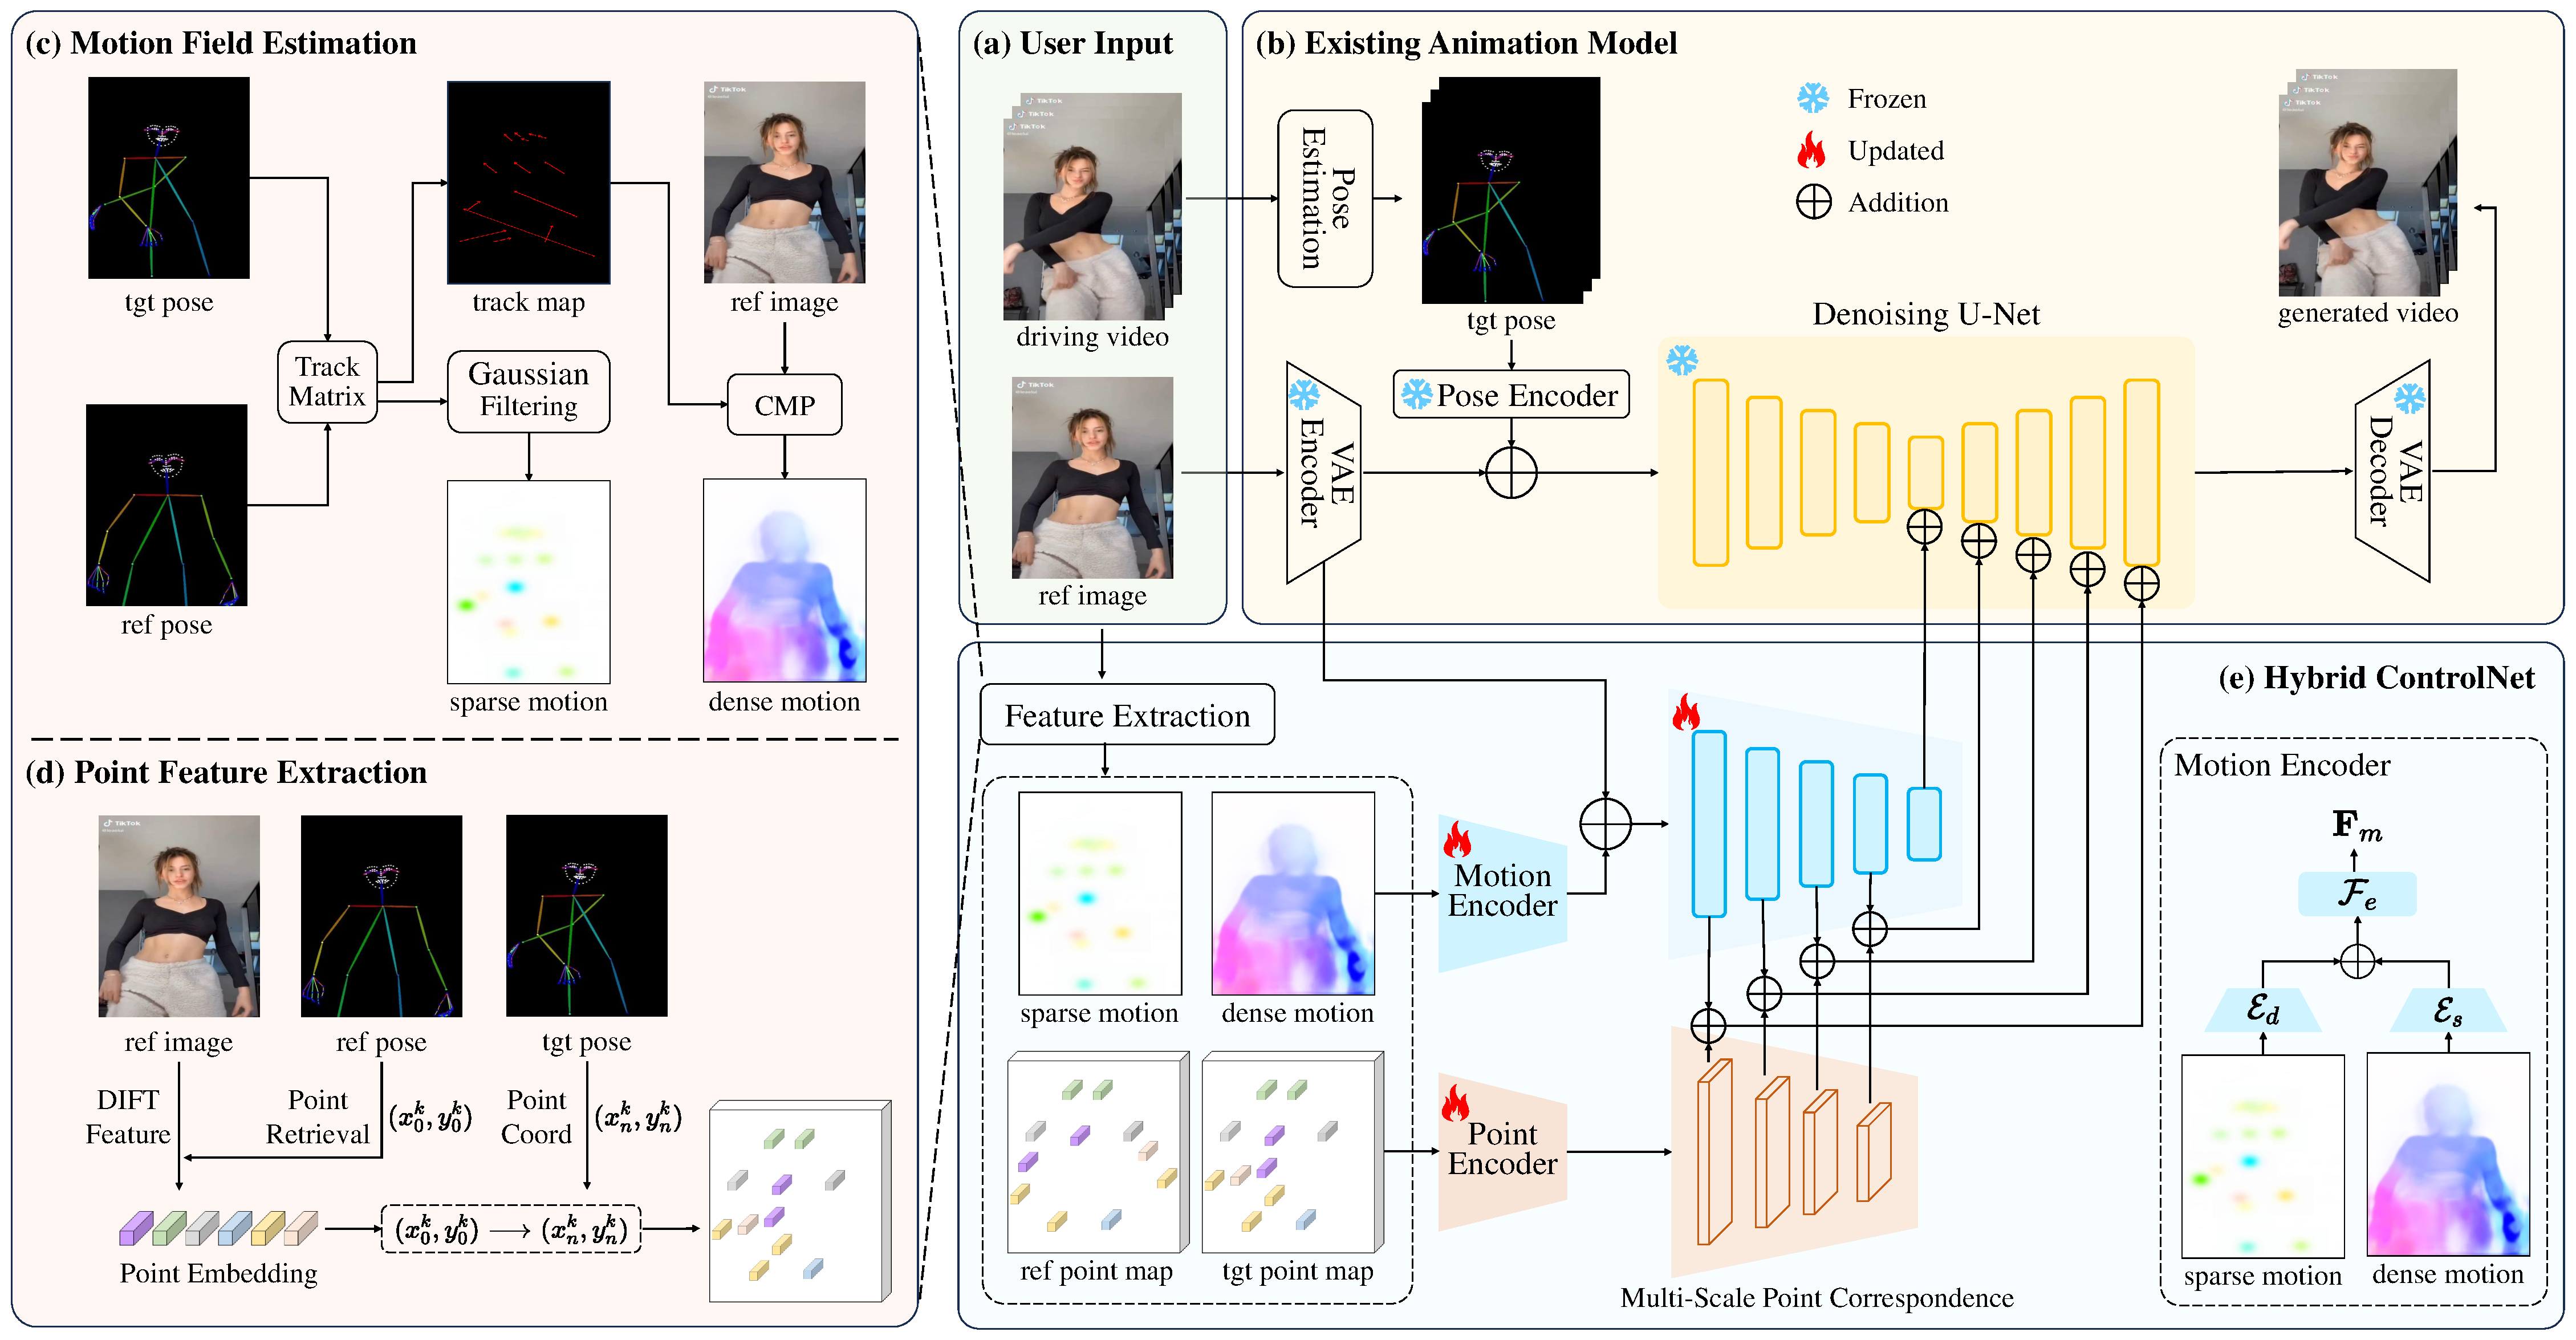
\includegraphics[width=1.0\columnwidth]{./image/pipeline.pdf}
    \vspace{-15pt}
    \caption{The overview of proposed DisPose.}
    \label{fig:pipeline}
\end{figure}
\section{DisPose}
Given a reference image $I_{\mathrm{ref}}\!\in\!\mathbb{R}^{3 \times H \times W}$ and a driving video $V\!\in\!\mathbb{R}^{N\times 3 \times H \times W}$. The core of our method is to disentangle efficient control guidance from only skeleton poses and reference images as shown in Figure~\ref{fig:pipeline}, which can be applied to existing human animation methods without additional dense inputs. We first introduce sparse and dense motion field guides in Sec.~\ref{sec: motion}. Then, we introduce reference-based keypoint correspondence in Sec.~\ref{sec: keypoint}. Finally, we introduce the pipeline of hybrid ControlNet in Sec~\ref{sec: controlnet}.
\subsection{Motion Field Guidance}
\label{sec: motion}

\textbf{Sparse Motion Field.}
We first estimate the skeleton pose by DWpose~\citep{yang2023dwpose} to obtain each frame's human key point coordinates. 
% Subsequently, the motion trajectory of all semantic points in the entire video is obtained and represented as
Subsequently, the key points of the reference image are used as starting points to track the motion displacement of all frames and represented as $P_{traj}\!=\!\{(x^k_n,y^k_n) \!\mid\! k=1\dots K, n=0\dots N\}$, where $P_{traj}$ denotes the trajectory map of the key point $k$ overall $N$ frames and $n = 0$ denotes the reference image. We calculate the track matrix $P_{s}$ as follows:
\begin{equation}
    \mathbf{P}_{s}=\{(x^k_n-x^k_{n-1}, y^k_n-y^k_{n-1}) \mid n=1\dots N\}\},
\end{equation}
% where $P_{t}$ denotes the trajectory map of the key point point $k$ over all $N$ frames, and the reference frame when $n = 0$.
where $K$ denotes the number of keypoints, $N$ denotes the number of frames, $\mathbf{P}_{s}$ denotes the trajectory map of keypoint k over all N frames, and $n = 0$ denotes the reference image.
To avoid training instability caused by overly sparse trajectory matrice, we then apply Gaussian filtering to enhance $\mathbf{P}_{s}$ to obtain the sparse motion field $\mathbf{F}_s\!\in\!\mathbb{R}^{(N-1)\times 2 \times H \times W}$ inspired by~\citep{yin2023dragnuwa, wang2024motionctrl}.

\textbf{Dense Motion Field.}
Considering that sparse control provides limited guidance and dense control is hard to obtain during inference,
% For the dense motion field, 
we transform dense guidance into the motion propagation from the reference frame to the target pose, instead of the dense signal of the target pose. Specifically, in the inference, we reconstruct the trajectory map $\mathbf{P}_{s}$ as the reference-based sparse optical flow $\mathbf{P}_{d}$ from the reference frame to each target pose as:
\begin{equation}
    \mathbf{P}_{d}=\{(x^k_n-x^k_{0}, y^k_n-y^k_{0}) \mid n=1\dots N\}\},
\end{equation}
We then predicted the reference-based dense motion filed $\mathbf{F}_d\!=\! \text{CMP}(P_{traj}, \mathbf{P}_{d}, I_{ref})\!\in\!\mathbb{R}^{(N-1)\times 2 \times H \times W}$ by condition motion propagation (CMP)~\citep{zhan2019self} based on the sparse optical flow $\mathbf{P}_{d}$ and the reference image $I_{ref}$.
CMP~\citep{zhan2019self} is a self-supervised learning-from-motion model that acquires an image and a sparse motion field and estimates the corresponding dense motion field.
Notably, the dense motion field $\mathbf{F}_d$ of each frame starts with the reference image, which avoids geometric constraints during inference.

To ensure motion estimation accuracy during training, we first extract the forward optical flow from the driving video using existing optical flow estimation models~\citep{teed2020raft, xu2023unifying}. We then use a watershed-based approach~\citep{zhan2019self} to sample the sparse optical flow $\mathbf{P}_{d}$ from the forward optical flow. See Appendix.~\ref{sec: appendix1} for details.

\textbf{Motion Encoder.} To leverage motion field as guidance, we introduce a motion encoder specifically designed for the optional flow, which includes sparse motion encoder $\mathcal{E}_s$, dense motion encoder $\mathcal{E}_d$ and feature fusion layer $\mathcal{F}_e$. $\mathcal{E}_d$ and $\mathcal{E}_s$ have the same structure and are multi-scale convolutional encoders with each stage built by \texttt{Conv-SiLU-ZeroConv}~\citep{zhang2023adding} as the basic block. The feature fusion layer $\mathcal{F}_e$ is a 2D convolution for fusing sparse motion features $\mathcal{E}_s(\mathbf{F}_s)$ and dense motion features $\mathcal{E}_d(\mathbf{F}_d)$. Finally, we compute the motion field guidance $\mathbf{F}_m$:
\begin{equation}
    \mathbf{F}_m = \mathcal{F}_e(\mathcal{E}_s(\mathbf{F}_s)+\mathcal{E}_d(\mathbf{F}_d))
\end{equation}

\subsection{Keypoint Correspondence}
\label{sec: keypoint}
\textbf{Point Feature Extraction.} 
To maintain a consistent appearance, it is crucial to correspond the content of the reference image with the motion trajectory. 
Specifically, we first extract the DIFT~\citep{tang2023emergent} features $\mathbf{D}$ of the reference image using the pre-trained image diffusion model. 

Subsequently, the keypoint embedding in the reference is obtained as $\mathbf{D}(x^k_0,y^k_0)$, where $(x^k_0,y^k_0)$ is retrieved from the reference pose.
% key point embeddings $\mathbf{D}(x^k_0,y^k_0)$ are retrieved from $\mathbf{D}$ by skeleton pose $(x^k_0, y^k_0)$.
Next, we initialize the keypoint correspondence map $\mathbf{F}_p$ with zero vectors and assign point embeddings according to the trajectory coordinates as:
\begin{equation}
\label{eq: v prob}
f^{ij}_n=\left\{\begin{array}{ll}
\mathbf{D}(x^k_0,y^k_0), & \mathrm{if} \quad i=x^k_n, j=y^k_n,  \\
0, & \mathrm{otherwise}.
\end{array}\right.
\end{equation}

Finally, we obtain the keypoint correspondence map $\mathbf{F}_p=\{f_n\!\mid\!n=1\dots N\} \!\in\!\mathbb{R}^{N\times D_p \times H \times W}$ for all frames, where $D_p$ is the feature dimension of the point embedding.

\textbf{Point Encoder.} 
To utilize the content correspondence of key points as guidance, we generate multi-scale correspondences of sparse point feature maps and make them compatible with the U-Net encoder of the {Hybrid ControlNet (Sec.4.3)}. 
% as detailed in F. 1.
We introduce the multi-scale point encoder $\mathcal{E}_p$ to maintain the key point content $\mathbf{F}_p$ from the reference image. The point encoder $\mathcal{E}_p$ consists of a series of learnable MLPs.
{
To seamlessly integrate into existing models, we extract intermediate features of the encoder of the hybrid Controlnet.
The multi-scale intermediate features of the Controlnet encoder are denoted as $\mathbf{E}^l_{enc}$, where $l$ denotes each U-Net block $l\!\in\![1, L]$.}
To match the spatial size of $\mathbf{E}^l_{enc}$, we apply downsampling to the feature map between the encoder layers. We compute the multi-scale keypoint correspondence as follows:
\begin{equation}
    \mathbf{F}_c^l = \mathcal{E}_p^l(\phi(\mathbf{F}_p, H^l, W^l)),
\end{equation}
where $(H^l, W^l)$ are denote the spatial dimension of the $l$-th U-Net block and $\phi$ means downsampling operation. Therefore, $\mathbf{F}_c^l$ shares the same size as $\mathbf{E}^l_{enc}$.
Finally, $\mathbf{F}_c$ are added elementwisely to the intermediate feature $\mathbf{E}^l_{enc}$ of the U-Net encoder as guidance: $\mathbf{E}^l_{enc}\!=\!\mathbf{E}^l_{enc}+\mathbf{F}_c^l$.


\subsection{Plug-and-play Hybrid ControlNet}
\label{sec: controlnet}
After obtaining motion field guidance and keypoint correspondence, we aim to integrate these control guidance seamlessly into the U-Net architecture of existing animation models.
Inspired by ControlNet~\citep{zhang2023adding}, We design a hybrid ControlNet $\mathcal{F}$ to provide additional control signals for the existing animation model as shown in Figure~\ref{fig:pipeline}(e).
% Specifically, we consider freeze denoising U-Net and pose encoder. 
Specifically, given an animation diffusion model based on the U-Net architecture, we freeze all its modules while allowing the motion encoder, point encoder and hybrid ControlNet to be updated during training. 
Subsequently, $\mathbf{F}_m$ is added to the noise latent before being input into the hybrid ControlNet. Considering the high sparsity of the point feature $\mathbf{F}_c$, we correspondingly add $\mathbf{F}_c$ to the input of the convolutional layer. Notably, the U-Net encoder intermediate feature $\mathbf{E}_{enc}$ in Sec.~\ref{sec: keypoint} is from hybrid ControlNet rather than denoising U-Net. Finally, 
the control condition is computed as:
\begin{equation}
    \boldsymbol{r}=\mathcal{F}(\boldsymbol{z}_{{t}} \mid \mathbf{F}_m, \mathbf{F}_c, {t})
\end{equation}
where $\boldsymbol{r}$ is a set of condition residuals added to the residuals for the middle and upsampling blocks in the denoising U-Net.
\section{Experiments} \label{sec:experiments}


\begin{table*}[t]
% \setlength\tabcolsep{3pt}  %可以控制列间距
% \renewcommand{\arraystretch}{1.1} %可以控制行间距
% \footnotesize
\centering
\fontsize{9}{11}\selectfont
\setlength{\tabcolsep}{2.6mm}{
\begin{tabular}{c|l|cccccc}
\toprule
\multicolumn{1}{c|}{\multirow{2}{*} {Type}} & \multicolumn{1}{l|}{\multirow{2}{*} {Model}}   & \multicolumn{3}{c}{WebQSP}   & \multicolumn{3}{c}{CWQ} \\
\cline{3-8}
 \multicolumn{1}{c|}{} & \multicolumn{1}{c|}{}   &F1&Hits@1& Acc &F1&Hits@1& Acc\\ 
\hline
\hline
\multicolumn{1}{c|}{\multirow{4}{*} {EM-based}} & KV-Mem {\scriptsize \cite{miller2016key}} & 34.5 & 46.7 & - & 15.7 & 18.4 & - \\
\multicolumn{1}{c|}{}& NSM$_{+h}$ {\scriptsize \cite{NSM}} &67.4 & 74.3& - & 44.0& 48.8&-   \\
\multicolumn{1}{c|}{}& TransferNet {\scriptsize \cite{shi2021transfernet}} &-  & 71.4 &- &- &48.6 &  - \\
\multicolumn{1}{c|}{}& KGT5 {\scriptsize \cite{KGT5}} &-  &56.1 &- &- & 36.5&  - \\
\hline
\multicolumn{1}{c|}{\multirow{5}{*} {IR-based}} &  GraftNet {\scriptsize \cite{sun-etal-2018-open}} & 60.4 & 66.4 & - & 32.7 & 36.8 & - \\
\multicolumn{1}{c|}{}& PullNet {\scriptsize \cite{sun-etal-2019-pullnet}} & - & 68.1 & - & - &45.9 & - \\
\multicolumn{1}{c|}{}& SR+NSM {\scriptsize \cite{zhang2022subgraph}} &  64.1 & 68.9 &- &47.1& 50.2&- \\
\multicolumn{1}{c|}{}& SR+NSM+E2E {\scriptsize \cite{zhang2022subgraph}} & 64.1  &69.5 &- &46.3&49.3 &-\\
\multicolumn{1}{c|}{}& UniKGQA {\scriptsize \cite{unikgqa}} & 71.0 &77.0& - &49.4& 50.9 &-\\
\hline
\multicolumn{1}{c|}{\multirow{6}{*} {SP-based}}& CBR-KBQA {\scriptsize \cite{CBR-KBQA}} & 72.8 &- &69.9 &70.0 &-& 67.1 \\
\multicolumn{1}{c|}{}& GMT-KBQA {\scriptsize \cite{GMT-KBQA}} & 76.6 &- &73.1 &77.0 &-& 72.2 \\
\multicolumn{1}{c|}{}& UnifiedSKG {\scriptsize \cite{xie-etal-2022-unifiedskg}} & 73.9 &-& -& 68.8& - &-\\
\multicolumn{1}{c|}{}& RnG-KBQA {\scriptsize \cite{rng-kbqa}} & 75.6&-&-&-&-&-\\
\multicolumn{1}{c|}{}& DecAF {\scriptsize \cite{decaf}} & 78.8&82.1&-&-&70.4&-\\
\multicolumn{1}{c|}{}& FC-KBQA {\scriptsize \cite{fc-kbqa}} & 76.9& - &- &56.4& -& -\\
\hline
\multicolumn{1}{c|}{\multirow{8}{*} {LLM-based}} & KD-CoT {\scriptsize \cite{wang2023knowledge}} & 52.5 & 68.6 & - &-  &55.7 & - \\
\multicolumn{1}{c|}{}& Pangu {\scriptsize \cite{pangu}} & 79.6 & - & - & - & - & - \\
\multicolumn{1}{c|}{}& StructGPT {\scriptsize \cite{structgpt}} & - & 72.6 & -  & -  & - & - \\
\multicolumn{1}{c|}{}& ChatKBQA {\scriptsize \cite{chatkbqa}} & 79.8 &83.2& 73.8 &77.8 &82.7 &73.3\\
\multicolumn{1}{c|}{}& ToG-R (GPT-4) {\scriptsize \cite{TOG}} & - & 82.6 & -  & -  & 69.5 & - \\
\multicolumn{1}{c|}{}& G-Retriever {\scriptsize \cite{G-retriever}} & -& 70.1& -& -& -& -\\
\multicolumn{1}{c|}{}& GNN-RAG {\scriptsize \cite{mavromatis2024gnn}} & 73.5 &82.8& -  &60.4& 62.8& - \\
\rowcolor{gray!10}  \multicolumn{1}{c|}{}& \model (Ours) & \textbf{81.2}\scriptsize{$\pm$0.15} & \textbf{84.3}\scriptsize{$\pm$0.16}  & \textbf{75.2}\scriptsize{$\pm$0.10} & \textbf{78.5}\scriptsize{$\pm$0.11} & \textbf{83.1}\scriptsize{$\pm$0.09} & \textbf{74.5}\scriptsize{$\pm$0.07} \\
\bottomrule
\end{tabular}}
\caption{Performance comparison of different types of KGQA methods on WebQSP and CWQ datasets. We present the Mean scores and standard deviations (mean ± std) of five experiments with different random seeds. The best result is highlighted in \textbf{bold}, and the baseline results are taken from corresponding papers.}
\label{tab:main result}
\end{table*}



\subsection{Experiment Settings}

\textbf{Datasets. }
Our experiments were conducted using two well-known datasets: WebQuestionsSP (WebQSP) \cite{webqsp} and ComplexWebQuestions (CWQ) \cite{CWQ}. The dataset statistics are presented in the Appendix. 
Both datasets contain SPARQL queries that correspond to the questions and can be executed on Freebase to obtain answers.

\noindent\textbf{Baselines.}
In this study, we evaluate performance with 22 baselines, which are categorized into four groups: embedding-based (EM-based), information retrieval-based (IR-based), semantic parsing-based (SP-based), and LLM-based methods. For more detailed descriptions of the baselines, please refer to the Appendix.
It is important to note that some methods, such as DecAF~\cite{decaf}, can be classified as multiple groups, specifically IR-based and SP-based. To ensure fairness, we do not include the results of using the oracle entity linking annotations setting, such as RoG \cite{RoG}. We put the performance comparison of the oracle setting in the Appendix.





\noindent\textbf{Evaluation Metrics.}
We use Hits@1, F1, and Acc as primary evaluation metrics following \cite{chatkbqa}. Hits@1 assesses the accuracy of top-1 predicted answer, F1 considers the coverage of all possible answers, and Acc measures the strict exact-match accuracy.
We further assess the quality of generated S-expressions by employing two metrics: the extract match ratio (EM) and the match after beam search ratio (BM) with ground-truth S-expressions, for analytical experiments.

\noindent\textbf{Implementation Details.}
% We employ LLaMA2-7B and LLaMA2-13B \cite{touvron2023llama} as LLM backbones, and then fine-tune LLMs using LoRA \cite{hu2022lora} on WebQSP and CWQ. 
Following ~\citet{chatkbqa}, we fine-tune LLaMA2-7B on WebQSP and LLaMA2-13B on CWQ using LoRA.
We evaluate the impact of backbones and fine-tuning methods in our subsequent experiments. During inference, we utilize beam search to generate multiple logical forms. We select the executable logical form with the highest score to obtain answers. All experiments were done on NVIDIA A6000 GPUs. We only searched the number of retrievals $k$ with values of \{4,8,16,32,64,100\}. 

\subsection{Main Results}
% In this section, we compare our method with all baselines.
As observed from Table \ref{tab:main result}, \model outperforms all baselines across all metrics on both datasets. Notably, on WebQSP dataset, accuracy has improved by 1.6\% compared to the second-best baseline, ChatKBQA, marking new state-of-the-art performance.
Specifically, \model surpasses subgraph retrieval techniques such as SR+NSM and DecAF with 26\% and 2.4\% F1 improvements on WebQSP, respectively, as well as entity and relation retrieval methods like GMT-KBQA with 5.3\% F1 improvement on WebQSP.
This can be attributed to our proposed self-alignment mechanism, which effectively aligns multi-aspect knowledge.
On the other hand, \model also outperforms other LLM-based approaches, such as G-Retriever and ChatKBQA, suggesting that our approach of learning prompt embeddings for retrieval can more flexibly leverage the capabilities of LLMs to utilize retrieval knowledge.


\begin{table}[t]
\setlength\tabcolsep{2pt}  %可以控制列间距
% \renewcommand{\arraystretch}{1.1} %可以控制行间距
\footnotesize
\centering
\fontsize{9}{11}\selectfont
\setlength{\tabcolsep}{3mm}
\begin{tabular}{l|ccccc}
\toprule
 \multicolumn{1}{l|}{\multirow{2}{*} {Model}} & \multicolumn{5}{c}{WebQSP} \\
\cline{2-6}
 \multicolumn{1}{c|}{} &F1&Hits@1& Acc & EM & BM  \\ 
\hline
\hline
\rowcolor{gray!10} \model & \textbf{81.2} & \textbf{84.3} & \textbf{75.2} & \textbf{63.9} & 76.4\\
w/o \textit{SN} & 80.1 & 83.3 & 74.3& 63.6 & \textbf{77.0}\\
w/o \textit{SA} & 79.5 & 82.6 & 73.8 & 63.0 &75.7 \\
w/o \textit{RG} &79.4 & 82.2 &74.3 & 63.4 & 76.7\\
w/o \textit{SA\&RG} & 78.7& 81.0 & 72.5  & 62.1 & 73.6 \\
w/o \textit{SA\&SN}	&79.1	&82.0	&73.8&	63.1&	76.2\\
w/o \textit{ALL} & 76.2 & 79.5 & 70.1 & 59.7 & 72.4  \\
\bottomrule
\end{tabular}
 \caption{Ablation study of sub-modules on WebQSP dataset.}
\label{tab:ablation}
\end{table}



\subsection{Ablation Study}
In this section, we conduct a series of ablation studies to address the following question: 

\textbf{How do the proposed modules improve performance?} Specifically, we conduct experiments against five variants:
1) w/o \textit{SN}: without siamese network, and relevance score is calculated by vector inner product; 2) w/o \textit{SA}: without self-alignment module; 3)  w/o \textit{RG}: without relevance gating module; 4) w/o \textit{SA\&RG}: without both self-alignment and relevance gating modules, where \model obtains prompt embeddings with only MLP. 5) w/o \textit{ALL}: directly appending the retrieval knowledge as context instead of converting retrieval knowledge to prompt embeddings.
As shown in Table \ref{tab:ablation}, we observe that the performance on most metrics decreases when either \textit{SN}, \textit{SA}, or \textit{RG} is removed. This validates the effectiveness of the proposed sub-modules. Furthermore, we find that performance significantly drops when the entire framework is removed, indicating that appending retrieved knowledge directly as context text introduces a large amount of noise, preventing LLMs from focusing on learning the mapping from question to logical form.
Additionally, we notice that the BM is higher in \model w/o \textit{SN} than in \model. This suggests that the ground-truth logical forms are mostly ranked within the top 2 or lower positions during beam search generation, leading to a lower EM.


\begin{table}[t]
% \setlength\tabcolsep{3pt}  %可以控制列间距
\renewcommand{\arraystretch}{1.1} %可以控制行间距
\footnotesize
\centering
\fontsize{9}{11}\selectfont
\setlength{\tabcolsep}{2.8mm}
\begin{tabular}{l|ccccc}
\toprule
 \multicolumn{1}{l|}{\multirow{2}{*} {Model}} & \multicolumn{5}{c}{WebQSP} \\
\cline{2-6}
 \multicolumn{1}{c|}{} &F1&Hits@1& Acc & EM & BM  \\ 
\hline
\hline
\rowcolor{gray!10} \model & \textbf{81.2} & \textbf{84.3} & \textbf{75.2} & \textbf{63.9} & \textbf{76.4} \\
w/o \textit{Relation} & 78.6 & 81.7 &73.1 & 63.0& 74.9\\
w/o \textit{Entity} & 79.2 & 82.2& 73.5& 63.8 & 74.4\\
w/o \textit{Subgraph} &79.7 &82.9 &73.8 & 63.5 & 75.1 \\
\bottomrule
\end{tabular}
 \caption{Quantitative comparison of the impacts of retrieval information on \model's performance.}
\label{tab:ablation retrieval}
\end{table}


\textbf{What impacts do different aspects of retrieval information have on performance?}
To preserve the integrity of \textsc{Amar}, we remove retrieval knowledge by replacing the text embedding with randomly initialized ones. As shown in Table \ref{tab:ablation retrieval}, the results indicate obvious performance drops after removing retrieval knowledge, including `\textit{subgraph}', `\textit{entity}', and `\textit{relation}'. This decline highlights the significance of different aspects of the retrieval knowledge on the overall performance.
Further analysis reveals that removing the `\textit{relation}' component results in the largest drop in performance, suggesting that `\textit{relation}' plays a crucial role in generating logical expressions. Instead, while the `\textit{subgraph}' still contributes to performance, it appears to be less critical for logical forms than `\textit{relation}' or `\textit{entity}'. These findings provide valuable insights for further optimization of the model.

\subsection{Number of Retrieval Analysis}
In this section, we explore the impact of the number of retrieval knowledge. We compare the approach of directly inputting retrieved data as a \textit{context prompt}. If the input exceeds the maximum context limit (i.e., 4096 for LLaMA2), we truncate the retrieved information from subgraphs. As shown in figure \ref{fig:topk}, it can be observed that when the amount of retrieved data is relatively small, our method does not significantly differ from  \textit{Context Prompt}, which suggests that useful information recalled is still limited.
However, as the quantity of retrieved data increases (e.g., reaching 64 or 100), our method achieves a substantial performance improvement, while \textit{context prompt} drastically declines. This demonstrates that introducing a long context results in substantial noise, making it difficult for LLMs to learn important data.
In contrast, by treating retrieved information as an individual prompt embedding, we avoid the issue of excessively long inputs and better utilize the rich information.



\begin{figure}[t]
\centering
\begin{minipage}[c]{0.225\textwidth}
    \centering
    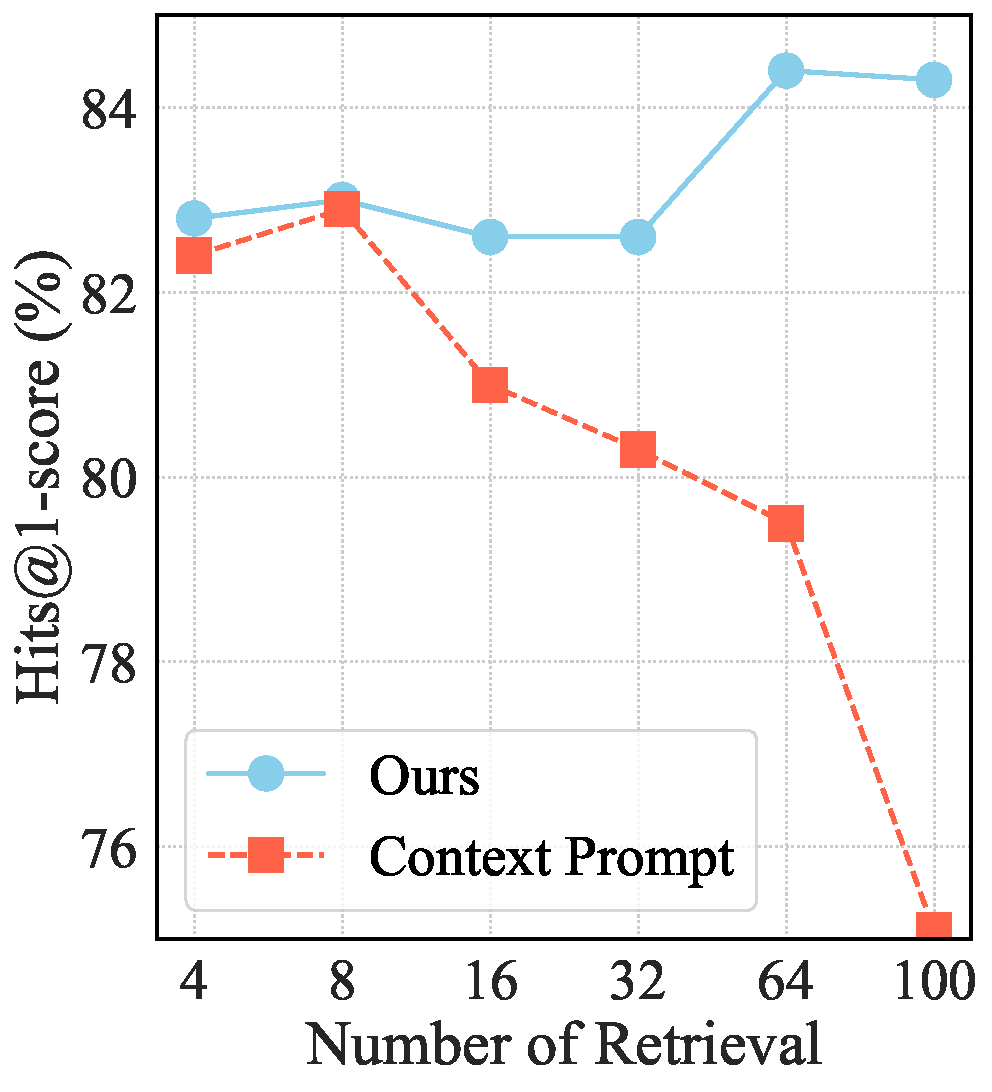
\includegraphics[width=\textwidth]{img/hyperparamter.pdf}
    \caption{Performance vary with the number of Retrieval.}
    \label{fig:topk}
\end{minipage}
\begin{minipage}[c]{0.225\textwidth}
    \centering
    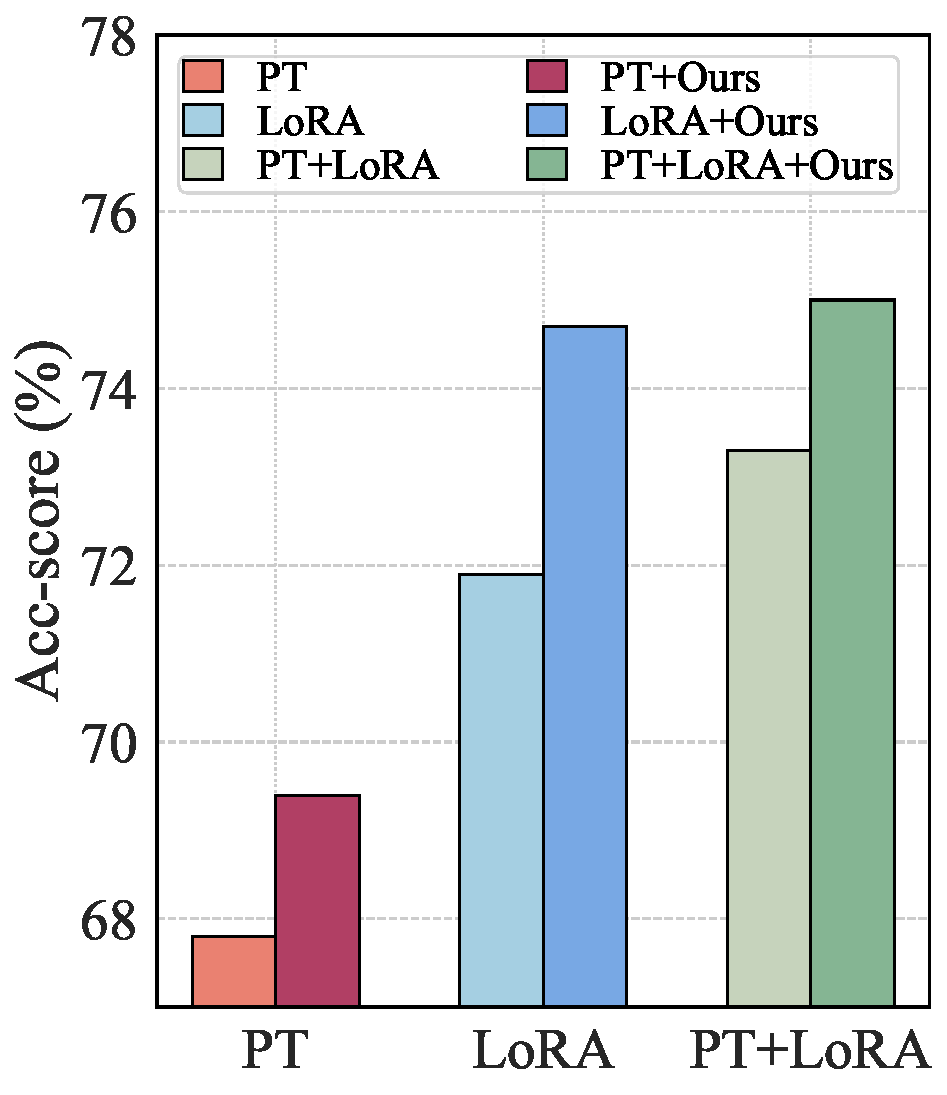
\includegraphics[width=\textwidth]{img/bar.pdf}
    \caption{Combine with different fine-tuning methods.}
    \label{fig:Tuning}
\end{minipage} 
\end{figure}

\begin{table*}[t]
% \setlength\tabcolsep{3pt}  %可以控制列间距
% \renewcommand{\arraystretch}{0.8} %可以控制行间距
\centering
\footnotesize
\begin{tabular}{p{2.7cm}p{14cm}}
\toprule
Question & \textit{what highschool did harper lee go to?} \\
\midrule 
Entity Retrieval & \textit{\ding{172} Harper Lee {[0.9272]}, \ding{173} Senior secondary education {[0.5441]}, 
 \ding{174} Lee Remick {[0.6482]}, \ding{175} Secondary education {[0.5412]}, \ding{176} Barbara Kingsolver {[0.4320]}, \ding{177} High school movement {[0.6758]}}  \\
 \midrule 
Relation Retrieval &  \textit{\ding{172}  people.person.education {[0.9844]},  \ding{173} education.education.institution {[0.9844]},  \ding{174} education.educational\_institution.school\_type {[0.7281]}, \ding{175} education.school.lowest\_grade\_taught {[0.5469]},  \ding{176} education.school\_mascot.school {[0.5431]}, \ding{177} common.topic.notable\_types {[0.8252]}} \\
\midrule 
 Logical Form by \model & \textit{(AND (JOIN common.topic.notable\_types High school) (JOIN (R education.education.institution) (JOIN (R people.person.education) Harper Lee)))} { \CheckmarkBold} \\
\midrule 
 Logical Form by Context Prompt  & \textit{(AND (JOIN \underline{education.educational.institution.school\_type} \underline{School}) (JOIN (R education.education.institution) ( JOIN (R people.person.education) Harper Lee)))} { \XSolidBrush} \\
\bottomrule 
\end{tabular}
\caption{A case study on WebQSP, where the `\textit{[float]}' represents the scores assigned to each retrieval information, indicating the level of influence it has on the model and the \underline{text with underline} means erroneous generation.
}
\label{tab:case}
\end{table*}

\subsection{Efficiency of Fine-Tuning}

In this section, we analyze the efficiency of our method combined with different fine-tuning methods, including Prompt Tuning (PT)~\cite{lester2021prompttuning} and Low-Rank Adaptation (LoRA). To ensure fairness, we conduct fine-tuning experiments without our module by concatenating the retrieved knowledge text with the input context. As shown in Figure \ref{fig:Tuning}, we observe a significant improvement in performance after incorporating \textsc{Amar}, Regardless of whether PT or LoRA is used, our method consistently outperforms baselines.  Notably, the combination of our method with PT+LoRA fine-tuning yields the best results. This highlights the capability of \model to effectively learn from retrieved information, while the direct concatenation of context introduces considerable noise.
Furthermore, we find that LoRA fine-tuning outperforms PT fine-tuning. This can be attributed to the inherent complexity of logical form generation in the KGQA task.  
LoRA has more tunable parameters and can act on all project layers, thus enabling LLMs to better adapt to tasks.


\subsection{Case Study}


In this section, we present a case study to illustrate how our model adaptively learns the importance of retrieval knowledge. We have not presented a case for subgraph retrieval due to its extensive length. As shown in Table \ref{tab:case}, our method is proven effective in assigning high scores to correct entities and relations for entity retrieval and relation retrieval, while irrelevant or misleading information receives low scores. For instance, the entity `\textit{Harper Lee}' received a score of [0.9272], and relation `\textit{people.person.education}' received a score of [0.9844].
Nevertheless, when retrieved text is directly used as the context prompt, it is susceptible to interference from erroneous information in retrieved data. This can result in generating incorrect relations, such as `\textit{education.educational.institution.school type}'. This example highlights that our method not only enhances the performance of LLM in KGQA but also improves the quality of retrieved information by setting weight.

        

\subsection{Analysis of LLM Backbones}
In this section, we investigate the question: \textbf{Does the performance improvement of our method solely come from LLMs?} To answer this, we conduct experiments and compare results using different LLMs as backbones: LLaMA2-7B with fine-tuning, LLaMA2-13B with fine-tuning, and GPT-4 (frozen).
% We observe that when using both LLama2-7b and 13b as backbones, \model outperforms baselines using the same backbone, even better than ToG-R~\cite{TOG} using GPT-4.
In Table \ref{tab:llms}, we observe that \model with LLaMA2-7B and 13B as backbones outperform the baselines using the same backbone, such as ChatKBQA~\cite{chatkbqa}, and both even surpass ToG-R~\cite{TOG} using GPT-4 as the backbone on two datasets.
% Moreover, experiments with LLaMA2-7B even reach slightly better results than with LlaMA2-13B on WebQSP because of over-fitting.
These results suggest that the performance gain of \model is not solely attributed to the use of more capable LLMs but rather to the proposed utilization of the commonality between multi-aspect knowledge and the relevance of the question.
We found that LLaMA2-13B perform worse than LLaMA2-7B on WebQSP. We believe the reason lies in dataset characteristics: the scale of WebQSP (1) is much smaller than that of CWQ, and (2) WebQSP has a maximum complexity, only consisting of 2-hop questions. This may cause the LLaMA2-13B to overfit, leading to reduced performance.


\begin{table}[t]
% \setlength\tabcolsep{3pt}  %可以控制列间距
% \renewcommand{\arraystretch}{1.1} %可以控制行间距
\fontsize{9}{11}\selectfont
\centering
\setlength{\tabcolsep}{3.7mm}{
\begin{tabular}{l|cccc}
\toprule
 \multicolumn{1}{l|}{\multirow{2}{*} {Model}}   & \multicolumn{2}{c}{WebQSP}  & \multicolumn{2}{c}{CWQ}     \\
\cline{2-5}
 \multicolumn{1}{c|}{}   &Acc &Hits@1 &Acc&Hits@1 \\ 
  \hline
  \multicolumn{5}{c}{\textit{GPT-4}} \\
\hline
 ToG-R &- &82.6 &-  & 69.5\\
\hline
\multicolumn{5}{c}{\textit{LLaMA2-7B}} \\
\hline
G-Retriever & - & 70.1& - & - \\
GNN-RAG  &-  & 82.8& -& 62.8\\
ChatKBQA & 73.8 & 83.2 & 73.0 & 82.3 \\
\rowcolor{gray!10}  \model & \textbf{75.2} &\textbf{84.3} & 73.4 & 82.9 \\
 \hline
 \multicolumn{5}{c}{\textit{LLaMA2-13B}} \\
\hline
ChatKBQA & 73.1 & 82.7 & 73.3 & 82.7 \\
\rowcolor{gray!10}  \model & 74.7  &83.3 &\textbf{ 74.5} & \textbf{83.1}\\
\bottomrule
\end{tabular}}
 \caption{Analysis on different LLM backbones. }
\label{tab:llms}
\end{table}



% Answer : Monroe County High School




 
\section{Related Work} \label{sec:relatedwork}


\noindent
\textbf{Knowledge Graph Question Answering (KGQA).}
KGQA aims to answer questions over KG, and previous methods are usually categorized as EM-based, IR-based, SP-based and LLM-based methods.
EM-based methods encode the entities and relations in the embedding space and reason final answer using these structural embeddings~\cite{shi2021transfernet}.
% For instance, QA-GNN~\cite{yasunaga2021qa} utilizes graph neural networks (GNNs) to reason both KG subgraphs and QA contexts jointly.
IR-based KBQA methods propose to retrieve and re-rank answers from KGs given information conveyed in the question~\cite{chen2019uhop,zhang2022subgraph}.
SP-based methods, focus on transforming question into a structural query, such as SPARQL and S-expression, and reason final answers using these executable queries~\cite{liang2017neural,lan2020query}.
Besides, recent attempts have been made to utilize LLM-based methods for KGQA~\cite{jiang2023unikgqa,chenplan}.
For instance, \citet{RoG} presents a planning-retrieval-reasoning pipeline. ToG \cite{TOG} proposes to interactively explore paths and reasoning on KGs using LLM as an agent.
% G-Retriever is a retrieval-augmented method for general textual graphs and it integrates graph neural networks and LLMs via soft prompting~\cite{G-retriever}.
Despite their significant improvements, a substantial challenge persists when handling multi-aspect retrieved data as input, which may introduce irrelevant knowledge.
However, our method is capable of aligning knowledge and implementing adaptive relevance gating with questions, thus addressing this issue.


% \noindent
% \textbf{Parameter-Efficient Fine-Tuning (PEFT).}
% % 参考 G-Retriever, 简单介绍 lora  和 prompt tuning 等方法。
% Fine-tuning (FT) can provide additional knowledge to LLMs and adjust LLMs' input and output to, for example, adapt to the structured data. Various parameter-efficient fine-tuning (PEFT) methods have been proposed to refine LLMs with minimal training costs~\cite{hu2022lora,zhang2023adalora,li2021prefix,lester2021prompttuning}.
% Low-Rank Adaptation (LoRA) reduces the number of trainable parameters by decomposing a large matrix into two smaller low-rank matrices in the attention layers~\cite{hu2022lora}, and AdaLoRA improves on LoRA by adaptively allocating the parameters among different weight matrices and layers according to their importance scores~\cite{zhang2023adalora}.
% Prompt tuning adds task-specific prompts to the tuning data and these prompt parameters are updated during fine-tuning~\cite{lester2021prompttuning}.
% Prefix tuning is proposed to prefix task-specific vectors to the tuning data and only updates these prefix parameters while keeping the LLM's parameters frozen~\cite{li2021prefix}.

% However, PEFT methods, such as LoRA and Prompt tuning, may face difficulties in effectively utilizing the extensive information derived from long texts, which often yield subpar model performance \cite{chen2023longlora}. In contrast, our model designed an adaptive framework for the retrieval information, enabling efficient learning the mapping between knowledge to generate the desired output.


\noindent
\textbf{Large Language Model Reasoning.}
Considering the impressive abilities of LLMs, some previous works focus on facilitating LLMs' reasoning via prompting~\cite{NSM,CBR-KBQA,structgpt,wang2023knowledge,li2024visualization,10.1007/978-981-97-7232-2_18,chen2024tackling}.
% For example, as a neuro-symbolic approach, CBR-KBQA reuses existing cases to improve reasoning on unseen cases~\cite{CBR-KBQA}.
To overcome the unfaithful reasoning of LLMs, ~\citet{structgpt} proposes StructGPT, an iterative reading-then-reasoning framework, to improve reasoning of LLMs when handling structured data.
 % FAME leverages Monte-Carlo planning to generate faithful reasoning steps~\cite{hong2023faithful} and
KD-CoT is designed to formulate chain-of-thought into a multi-round QA format and LLMs can retrieve external knowledge during interaction~\cite{wang2023knowledge}.
% ~\citet{du2024improving} proposes to utilize multiple LLMs and obtain the final answer through discussion and debation among these LLMs, which improves the factual validity of the generated contents.
However, LLMs reasoning is challenging when leveraging information present in lengthy texts \cite{wang2024beyond}. In contrast, our model facilitates efficient selection of information by utilizing prompt embeddings, thereby mitigating the issue of excessive context.



Hyperbolic embeddings embed hierarchical information with high
fidelity and few dimensions. We explored the limits of this approach
by describing scalable, high quality algorithms. We hope the
techniques here encourage more follow-on work on the exciting
techniques of \citet{fb, ucl}. As future work, we hope to explore how
hyperbolic embeddings can be most effectively incorporated into downstream
tasks and applications.

\bibliography{aaai25}
% \newpage
\section*{NeurIPS Paper Checklist}

\begin{enumerate}

\item {\bf Claims}
    \item[] Question: Do the main claims made in the abstract and introduction accurately reflect the paper's contributions and scope?
    \item[] Answer: \answerYes{} 
    \item[] Justification: The abstract and the introduction both clearly state the claims made by the paper, along with a clear description of the contributions, assumptions and limitations. 
    \item[] Guidelines:
    \begin{itemize}
        \item The answer NA means that the abstract and introduction do not include the claims made in the paper.
        \item The abstract and/or introduction should clearly state the claims made, including the contributions made in the paper and important assumptions and limitations. A No or NA answer to this question will not be perceived well by the reviewers. 
        \item The claims made should match theoretical and experimental results, and reflect how much the results can be expected to generalize to other settings. 
        \item It is fine to include aspirational goals as motivation as long as it is clear that these goals are not attained by the paper. 
    \end{itemize}

\item {\bf Limitations}
    \item[] Question: Does the paper discuss the limitations of the work performed by the authors?
    \item[] Answer: \answerYes{}
    \item[] Justification: Yes, the limitations of the current work as well as the avenues for future improvements to the current work can be found in Section \ref{sec:disc}.
    \item[] Guidelines:
    \begin{itemize}
        \item The answer NA means that the paper has no limitation while the answer No means that the paper has limitations, but those are not discussed in the paper. 
        \item The authors are encouraged to create a separate "Limitations" section in their paper.
        \item The paper should point out any strong assumptions and how robust the results are to violations of these assumptions (e.g., independence assumptions, noiseless settings, model well-specification, asymptotic approximations only holding locally). The authors should reflect on how these assumptions might be violated in practice and what the implications would be.
        \item The authors should reflect on the scope of the claims made, e.g., if the approach was only tested on a few datasets or with a few runs. In general, empirical results often depend on implicit assumptions, which should be articulated.
        \item The authors should reflect on the factors that influence the performance of the approach. For example, a facial recognition algorithm may perform poorly when image resolution is low or images are taken in low lighting. Or a speech-to-text system might not be used reliably to provide closed captions for online lectures because it fails to handle technical jargon.
        \item The authors should discuss the computational efficiency of the proposed algorithms and how they scale with dataset size.
        \item If applicable, the authors should discuss possible limitations of their approach to address problems of privacy and fairness.
        \item While the authors might fear that complete honesty about limitations might be used by reviewers as grounds for rejection, a worse outcome might be that reviewers discover limitations that aren't acknowledged in the paper. The authors should use their best judgment and recognize that individual actions in favor of transparency play an important role in developing norms that preserve the integrity of the community. Reviewers will be specifically instructed to not penalize honesty concerning limitations.
    \end{itemize}

\item {\bf Theory Assumptions and Proofs}
    \item[] Question: For each theoretical result, does the paper provide the full set of assumptions and a complete (and correct) proof?
    \item[] Answer: \answerYes{} 
    \item[] Justification: Yes, for all the main results of the paper in Section \ref{sec:eigenspectrum_theory}, a full set of assumptions and a complete proof is provided in Section \ref{app:sec_proof} in the Appendix. 
    \item[] Guidelines:
    \begin{itemize}
        \item The answer NA means that the paper does not include theoretical results. 
        \item All the theorems, formulas, and proofs in the paper should be numbered and cross-referenced.
        \item All assumptions should be clearly stated or referenced in the statement of any theorems.
        \item The proofs can either appear in the main paper or the supplemental material, but if they appear in the supplemental material, the authors are encouraged to provide a short proof sketch to provide intuition. 
        \item Inversely, any informal proof provided in the core of the paper should be complemented by formal proofs provided in appendix or supplemental material.
        \item Theorems and Lemmas that the proof relies upon should be properly referenced. 
    \end{itemize}

    \item {\bf Experimental Result Reproducibility}
    \item[] Question: Does the paper fully disclose all the information needed to reproduce the main experimental results of the paper to the extent that it affects the main claims and/or conclusions of the paper (regardless of whether the code and data are provided or not)?
    \item[] Answer: \answerYes{} 
    \item[] Justification: Yes, the paper discloses all the necessary details about the implemented architectures used, hyperparameters for each setting, algorithm pseudocode and other experimental details to reproduce all the experiments in the paper. These details can be found in Section \ref{app:secB} in the Appendix.
    \item[] Guidelines:
    \begin{itemize}
        \item The answer NA means that the paper does not include experiments.
        \item If the paper includes experiments, a No answer to this question will not be perceived well by the reviewers: Making the paper reproducible is important, regardless of whether the code and data are provided or not.
        \item If the contribution is a dataset and/or model, the authors should describe the steps taken to make their results reproducible or verifiable. 
        \item Depending on the contribution, reproducibility can be accomplished in various ways. For example, if the contribution is a novel architecture, describing the architecture fully might suffice, or if the contribution is a specific model and empirical evaluation, it may be necessary to either make it possible for others to replicate the model with the same dataset, or provide access to the model. In general. releasing code and data is often one good way to accomplish this, but reproducibility can also be provided via detailed instructions for how to replicate the results, access to a hosted model (e.g., in the case of a large language model), releasing of a model checkpoint, or other means that are appropriate to the research performed.
        \item While NeurIPS does not require releasing code, the conference does require all submissions to provide some reasonable avenue for reproducibility, which may depend on the nature of the contribution. For example
        \begin{enumerate}
            \item If the contribution is primarily a new algorithm, the paper should make it clear how to reproduce that algorithm.
            \item If the contribution is primarily a new model architecture, the paper should describe the architecture clearly and fully.
            \item If the contribution is a new model (e.g., a large language model), then there should either be a way to access this model for reproducing the results or a way to reproduce the model (e.g., with an open-source dataset or instructions for how to construct the dataset).
            \item We recognize that reproducibility may be tricky in some cases, in which case authors are welcome to describe the particular way they provide for reproducibility. In the case of closed-source models, it may be that access to the model is limited in some way (e.g., to registered users), but it should be possible for other researchers to have some path to reproducing or verifying the results.
        \end{enumerate}
    \end{itemize}


\item {\bf Open access to data and code}
    \item[] Question: Does the paper provide open access to the data and code, with sufficient instructions to faithfully reproduce the main experimental results, as described in supplemental material?
    \item[] Answer: \answerYes{} 
    \item[] Justification: The paper includes the specific instructions to access the datasets used for all the experimentation. These can be found in Section \ref{app:secB} in the Appendix. The code for this project is released to the public. 
    \item[] Guidelines:
    \begin{itemize}
        \item The answer NA means that paper does not include experiments requiring code.
        \item Please see the NeurIPS code and data submission guidelines (\url{https://nips.cc/public/guides/CodeSubmissionPolicy}) for more details.
        \item While we encourage the release of code and data, we understand that this might not be possible, so “No” is an acceptable answer. Papers cannot be rejected simply for not including code, unless this is central to the contribution (e.g., for a new open-source benchmark).
        \item The instructions should contain the exact command and environment needed to run to reproduce the results. See the NeurIPS code and data submission guidelines (\url{https://nips.cc/public/guides/CodeSubmissionPolicy}) for more details.
        \item The authors should provide instructions on data access and preparation, including how to access the raw data, preprocessed data, intermediate data, and generated data, etc.
        \item The authors should provide scripts to reproduce all experimental results for the new proposed method and baselines. If only a subset of experiments are reproducible, they should state which ones are omitted from the script and why.
        \item At submission time, to preserve anonymity, the authors should release anonymized versions (if applicable).
        \item Providing as much information as possible in supplemental material (appended to the paper) is recommended, but including URLs to data and code is permitted.
    \end{itemize}


\item {\bf Experimental Setting/Details}
    \item[] Question: Does the paper specify all the training and test details (e.g., data splits, hyperparameters, how they were chosen, type of optimizer, etc.) necessary to understand the results?
    \item[] Answer: \answerYes{} 
    \item[] Justification: Yes, the paper uses standard data splits from publicly available benchmark sources and provides details regarding the choice of hyperparameters, optimizer and other decisions necessary for understanding the results. These details can be found in Section \ref{app:secB} in the Appendix.
    \item[] Guidelines:
    \begin{itemize}
        \item The answer NA means that the paper does not include experiments.
        \item The experimental setting should be presented in the core of the paper to a level of detail that is necessary to appreciate the results and make sense of them.
        \item The full details can be provided either with the code, in appendix, or as supplemental material.
    \end{itemize}

\item {\bf Experiment Statistical Significance}
    \item[] Question: Does the paper report error bars suitably and correctly defined or other appropriate information about the statistical significance of the experiments?
    \item[] Answer: \answerYes{} 
    \item[] Justification: Yes, the paper reports the error bars and other information about the statistical significance of the results in the Section \ref{sec:experiments} in the main paper. 
    \item[] Guidelines:
    \begin{itemize}
        \item The answer NA means that the paper does not include experiments.
        \item The authors should answer "Yes" if the results are accompanied by error bars, confidence intervals, or statistical significance tests, at least for the experiments that support the main claims of the paper.
        \item The factors of variability that the error bars are capturing should be clearly stated (for example, train/test split, initialization, random drawing of some parameter, or overall run with given experimental conditions).
        \item The method for calculating the error bars should be explained (closed form formula, call to a library function, bootstrap, etc.)
        \item The assumptions made should be given (e.g., Normally distributed errors).
        \item It should be clear whether the error bar is the standard deviation or the standard error of the mean.
        \item It is OK to report 1-sigma error bars, but one should state it. The authors should preferably report a 2-sigma error bar than state that they have a 96\% CI, if the hypothesis of Normality of errors is not verified.
        \item For asymmetric distributions, the authors should be careful not to show in tables or figures symmetric error bars that would yield results that are out of range (e.g. negative error rates).
        \item If error bars are reported in tables or plots, The authors should explain in the text how they were calculated and reference the corresponding figures or tables in the text.
    \end{itemize}

\item {\bf Experiments Compute Resources}
    \item[] Question: For each experiment, does the paper provide sufficient information on the computer resources (type of compute workers, memory, time of execution) needed to reproduce the experiments?
    \item[] Answer: \answerYes{} 
    \item[] Justification: Yes, the paper provides details about the compute resources, hardware and software needed to reproduce the experiments in Section \ref{app:secB} of the Appendix.
    \item[] Guidelines:
    \begin{itemize}
        \item The answer NA means that the paper does not include experiments.
        \item The paper should indicate the type of compute workers CPU or GPU, internal cluster, or cloud provider, including relevant memory and storage.
        \item The paper should provide the amount of compute required for each of the individual experimental runs as well as estimate the total compute. 
        \item The paper should disclose whether the full research project required more compute than the experiments reported in the paper (e.g., preliminary or failed experiments that didn't make it into the paper). 
    \end{itemize}
    
\item {\bf Code Of Ethics}
    \item[] Question: Does the research conducted in the paper conform, in every respect, with the NeurIPS Code of Ethics \url{https://neurips.cc/public/EthicsGuidelines}?
    \item[] Answer: \answerYes{} 
    \item[] Justification: Yes, the research conducted in this paper conforms in every respect, with the NeurIPS code of ethics. 
    \item[] Guidelines:
    \begin{itemize}
        \item The answer NA means that the authors have not reviewed the NeurIPS Code of Ethics.
        \item If the authors answer No, they should explain the special circumstances that require a deviation from the Code of Ethics.
        \item The authors should make sure to preserve anonymity (e.g., if there is a special consideration due to laws or regulations in their jurisdiction).
    \end{itemize}


\item {\bf Broader Impacts}
    \item[] Question: Does the paper discuss both potential positive societal impacts and negative societal impacts of the work performed?
    \item[] Answer: \answerYes{} 
    \item[] Justification: We discuss the potential positive and negative societal impacts of our work in Section \ref{app:broader_impact} of the Appendix. 
    \item[] Guidelines:
    \begin{itemize}
        \item The answer NA means that there is no societal impact of the work performed.
        \item If the authors answer NA or No, they should explain why their work has no societal impact or why the paper does not address societal impact.
        \item Examples of negative societal impacts include potential malicious or unintended uses (e.g., disinformation, generating fake profiles, surveillance), fairness considerations (e.g., deployment of technologies that could make decisions that unfairly impact specific groups), privacy considerations, and security considerations.
        \item The conference expects that many papers will be foundational research and not tied to particular applications, let alone deployments. However, if there is a direct path to any negative applications, the authors should point it out. For example, it is legitimate to point out that an improvement in the quality of generative models could be used to generate deepfakes for disinformation. On the other hand, it is not needed to point out that a generic algorithm for optimizing neural networks could enable people to train models that generate Deepfakes faster.
        \item The authors should consider possible harms that could arise when the technology is being used as intended and functioning correctly, harms that could arise when the technology is being used as intended but gives incorrect results, and harms following from (intentional or unintentional) misuse of the technology.
        \item If there are negative societal impacts, the authors could also discuss possible mitigation strategies (e.g., gated release of models, providing defenses in addition to attacks, mechanisms for monitoring misuse, mechanisms to monitor how a system learns from feedback over time, improving the efficiency and accessibility of ML).
    \end{itemize}
    
\item {\bf Safeguards}
    \item[] Question: Does the paper describe safeguards that have been put in place for responsible release of data or models that have a high risk for misuse (e.g., pretrained language models, image generators, or scraped datasets)?
    \item[] Answer: \answerNA{} 
    \item[] Justification: The paper uses publicly available datasets, and does not release any data or code that have a risk of misuse. 
    \item[] Guidelines:
    \begin{itemize}
        \item The answer NA means that the paper poses no such risks.
        \item Released models that have a high risk for misuse or dual-use should be released with necessary safeguards to allow for controlled use of the model, for example by requiring that users adhere to usage guidelines or restrictions to access the model or implementing safety filters. 
        \item Datasets that have been scraped from the Internet could pose safety risks. The authors should describe how they avoided releasing unsafe images.
        \item We recognize that providing effective safeguards is challenging, and many papers do not require this, but we encourage authors to take this into account and make a best faith effort.
    \end{itemize}

\item {\bf Licenses for existing assets}
    \item[] Question: Are the creators or original owners of assets (e.g., code, data, models), used in the paper, properly credited and are the license and terms of use explicitly mentioned and properly respected?
    \item[] Answer: \answerYes{} 
    \item[] Justification: We have appropriately cited the original owners of data and code which is used in the paper. 
    \item[] Guidelines:
    \begin{itemize}
        \item The answer NA means that the paper does not use existing assets.
        \item The authors should cite the original paper that produced the code package or dataset.
        \item The authors should state which version of the asset is used and, if possible, include a URL.
        \item The name of the license (e.g., CC-BY 4.0) should be included for each asset.
        \item For scraped data from a particular source (e.g., website), the copyright and terms of service of that source should be provided.
        \item If assets are released, the license, copyright information, and terms of use in the package should be provided. For popular datasets, \url{paperswithcode.com/datasets} has curated licenses for some datasets. Their licensing guide can help determine the license of a dataset.
        \item For existing datasets that are re-packaged, both the original license and the license of the derived asset (if it has changed) should be provided.
        \item If this information is not available online, the authors are encouraged to reach out to the asset's creators.
    \end{itemize}

\item {\bf New Assets}
    \item[] Question: Are new assets introduced in the paper well documented and is the documentation provided alongside the assets?
    \item[] Answer: \answerNA{} 
    \item[] Justification: The paper does not release any new assets. 
    \item[] Guidelines:
    \begin{itemize}
        \item The answer NA means that the paper does not release new assets.
        \item Researchers should communicate the details of the dataset/code/model as part of their submissions via structured templates. This includes details about training, license, limitations, etc. 
        \item The paper should discuss whether and how consent was obtained from people whose asset is used.
        \item At submission time, remember to anonymize your assets (if applicable). You can either create an anonymized URL or include an anonymized zip file.
    \end{itemize}

\item {\bf Crowdsourcing and Research with Human Subjects}
    \item[] Question: For crowdsourcing experiments and research with human subjects, does the paper include the full text of instructions given to participants and screenshots, if applicable, as well as details about compensation (if any)? 
    \item[] Answer: \answerNA{} 
    \item[] Justification: The paper does not involve crowdsourcing, nor research with human subjects.
    \item[] Guidelines:
    \begin{itemize}
        \item The answer NA means that the paper does not involve crowdsourcing nor research with human subjects.
        \item Including this information in the supplemental material is fine, but if the main contribution of the paper involves human subjects, then as much detail as possible should be included in the main paper. 
        \item According to the NeurIPS Code of Ethics, workers involved in data collection, curation, or other labor should be paid at least the minimum wage in the country of the data collector. 
    \end{itemize}

\item {\bf Institutional Review Board (IRB) Approvals or Equivalent for Research with Human Subjects}
    \item[] Question: Does the paper describe potential risks incurred by study participants, whether such risks were disclosed to the subjects, and whether Institutional Review Board (IRB) approvals (or an equivalent approval/review based on the requirements of your country or institution) were obtained?
    \item[] Answer: \answerNA{} 
    \item[] Justification: The paper does not involve crowdsourcing nor research with human subjects.
    \item[] Guidelines:
    \begin{itemize}
        \item The answer NA means that the paper does not involve crowdsourcing nor research with human subjects.
        \item Depending on the country in which research is conducted, IRB approval (or equivalent) may be required for any human subjects research. If you obtained IRB approval, you should clearly state this in the paper. 
        \item We recognize that the procedures for this may vary significantly between institutions and locations, and we expect authors to adhere to the NeurIPS Code of Ethics and the guidelines for their institution. 
        \item For initial submissions, do not include any information that would break anonymity (if applicable), such as the institution conducting the review.
    \end{itemize}

\end{enumerate}

\appendix

% \section{Claimed Emergent Abilities}
% \label{app:claimed_emergent_abilities}

% We compile the models, tasks and metrics that different papers have claimed reveal emergent abilities of large language models. This list may be incomplete or inaccurate, but represents a good faith attempt to compile this information. Note: quantifying model scale when an ability emerges is complicated by the fact that different papers report model scale differently, either as (a) number of parameters \cite{brown2020language, ganguli2022predictability}, (b) effective number of parameters \cite{srivastava2022beyond} or (c) training FLOPs \cite{wei2022emergent}.

% \begin{table}[h!]
%     \centering
%     \begin{tabular}{|l|c|c|c|}
%     \hline
%         Task & Model Families & Metric & Model Scale at Emergence \\
%         \hline
%         2-Digit Addition \cite{brown2020language} & GPT-3 & Accuracy & 13B Parameters\\
%         2-Digit Subtraction \cite{brown2020language} & GPT-3 & Accuracy & 13B Parameters\\
%         3-Digit Addition \cite{brown2020language, ganguli2022predictability} & GPT-3 & Accuracy & 175B Parameters\\
%         3-Digit Subtraction \cite{brown2020language} & GPT-3 & Accuracy & 175B Parameters\\
%         MMLU \cite{ganguli2022predictability} & GPT-3, Gopher & Accuracy & 200B, 300B Parameters\\
%         Program Synthesis \cite{ganguli2022predictability} & Google Internal & \% Samples Solving Task & 200B Parameters\\
%         Figure of Speech Detection \cite{srivastava2022beyond} & ? & ? & $\sim 10^{11}$ Effective Parameters \\
%         IPA Transliterate \cite{srivastava2022beyond, wei2022emergent} & LaMDA, GPT-3 & BLEU & $\sim 10^{23}, \sim 10^{23}$ Training FLOPs\\
%         Periodic Elements \cite{srivastava2022beyond} & ? & ? & ?\\
%         Modified Arithmetic \cite{srivastava2022beyond, wei2022emergent} & GPT-3, LaMDA & Accuracy & $\sim 10^{23}, \sim 10^{24}$ Training FLOPs\\
%         Repeat Copy Logic \cite{srivastava2022beyond} & ? & ? & $10^{11}$ Effective Parameters\\
%         Word Unscrambling \cite{srivastava2022beyond, wei2022emergent} & LaMDA & Exact Match & $\sim 10^{24}$ Training FLOPs\\
%         Persian QA \cite{wei2022emergent} & PaLM & Exact Match & $\sim 10^{24}$ Training FLOPs\\
%         Truthful QA \cite{wei2022emergent} & Gopher & Accuracy & $\sim 10^{23}$ Training FLOPs\\
%         Grounded Mappings \cite{wei2022emergent} & ? & ? & ?\\
%         Multi-task NLU \cite{wei2022emergent} & ? & ? & ?\\
%         Word in context \cite{wei2022emergent} & ? & ? & $\sim 10^{24}$ Training FLOPs\\
%         \hline
%     \end{tabular}
%     \newline
%     \caption{\textbf{Tasks, model families, metrics and number of parameters for emergent abilities.}}
%     \label{tab:my_label}
% \end{table}


% \section{Exponentiated Negative Cross Entropy Lower Bounds Accuracy}
% \label{app:acc_bound}

% Consider batch size $B$ with length $L$. During training i.e. with teacher-forcing, the per-token accuracy (averaged over batch index $b$ and sequence index $l$) is defined as:
% %
% \begin{align}
%     \text{Acc} &\defeq \frac{1}{B} \sum_b \frac{1}{L} \sum_l p(t_{bl}^* | t_{b, <l}^*)\\
%     &= \frac{1}{BL} \sum_{b, l} p(t_{bl}^* | t_{b, <l}^*)
% \end{align}

% The cross entropy (commonly averaged over the batch) is defined as:
% %
% \begin{align}
%     \mathcal{L}_{CE} &\defeq -\frac{1}{B} \sum_b \log p(t_{b 1}^*, ..., t_{b L}^*)\\
%     &= -\frac{1}{B} \sum_b \log \prod_l p(t_{b l}^*| t_{b, <l}^*)\\
%     &= -\frac{1}{B} \sum_{b, l} \log p(t_{bl}^* | t_{b, <l}^*)
% \end{align}

% To make the comparison between accuracy and cross entropy a little easier, let's normalize the cross entropy by the sequence length:
% %
% \begin{align}
%     \mathcal{L}_{CE/L} &\defeq \frac{1}{L}\mathcal{L}_{CE}\\
%     &=  -\frac{1}{BL} \sum_{b, l} \log p(t_{bl}^* | t_{b, <l}^*)
% \end{align}

% Recall that Jensen's inequality tells us that for any random variable $X$, $\log \mathbb{E}[X] \geq \mathbb{E}[\log X]$. The relationship between sequence-length-normalized cross entropy and accuracy is thus:
% %
% \begin{align}
%     -\mathcal{L}_{CE/L} = \frac{1}{BL} \sum_{b, l} \log p(t_{bl}^* | t_{b <l}^*) &\leq \log \frac{1}{BL} \sum_{b, l}  p(t_{bl}^* | t_{b <l}^*) = \log \text{Acc}\\
%     \exp(- \mathcal{L}_{CE/L}) &\leq \text{Acc}
% \end{align}

% Consequently, we see that driving the cross entropy loss to $0$ necessarily drives the accuracy to $1$.

% TODO: Can we use the second moment method to derive bounds on how (un)likely a subset of tokens are to deviate from the mean?


\section{Approximate Behavior of Metrics on Sequential Data}
\label{app:metric_scaling}

How do different metrics behave when used to measure autoregressive model outputs? Precisely answering this question is tricky and possibly analytically unsolvable, so we provide an approximate answer here.

Notationally, we consider $N$ test data of length $L$ (here, length is measured in tokens) with targets denoted $t_n \defeq (t_{n1}, t_{n2}, ... t_{nL})$, the autoregressive model has a true-but-unknown per-token error probability of $\epsilon \in [0, 1]$ and the model outputs prediction $\hat{t}_n \defeq (\hat{t}_{n1}, \hat{t}_{n2}, ... \hat{t}_{nL})$. This assumes that the model's per-token error probability is constant, which is empirically false, but modeling the complex dependencies of errors is beyond our scope.

\subsection{Per-Token Error Probability is Resolution-Limited}
\label{app:metric_scaling:resolution_limited}

Note that because we have $N$ test data, each of length $L$, our resolution for viewing the per-token error probability $\epsilon$ is limited by $1/NL$. 
Here, resolution refers to ``the smallest interval measurable by a scientific instrument; the resolving power."
To explain what resolution means via an example, suppose one wants to measure a coin's probability of yielding heads.
After a single coin flip, only two outcomes are possible (H, T), so the resolution-limited probability of heads is either $0$ or $1$.
After two coin flips, four outcomes are possible (HH, HT, TH, TT), so the resolution-limited probability of heads is now one of $0, 0.5, 1$.
After $F$ coin flips, we can only resolve the coin's probability of yielding heads up to $1/F$.
Consequently, we introduce a resolution-limited notation:
%
\begin{equation}
    \nint{a}_b \defeq \text{$a$ rounded to the nearest integer multiple of $1/b$}
\end{equation}

\subsection{Token Edit Distance}
\label{app:metric_scaling:token_edit_distance}

We first consider an adaptation of the Levenshtein (string edit) distance for models that function on tokens rather than characters, an adaptation we term the \textit{token edit distance}. The token edit distance between two token sequences $t_n, \hat{t_n}$ is defined as the integer number of additions, deletions or substitutions necessary to transform $t_n$ into $\hat{t}_n$ (or vice versa).

\begin{align}
    \text{Token Edit Distance}(t_n, \hat{t}_n)  &\defeq \text{Num Substitutions} + \text{Num. Additions} + \text{Num. Deletions}\\
    &= \sum_{\ell =1}^L \mathbb{I}[t_{n\ell} \neq \hat{t}_{n\ell}] + \text{Num. Additions} + \text{Num. Deletions}\\
    &\geq \sum_{\ell =1}^L \mathbb{I}[t_{n\ell} \neq \hat{t}_{n\ell}]
\end{align}

The expected token edit distance is therefore:

\begin{align}
    \mathbb{E}[\text{Token Edit Distance}(t_n, \hat{t}_n)] &\geq \mathbb{E}[\sum_{\ell =1}^L \mathbb{I}[t_{n\ell} \neq \hat{t}_{n\ell}]]\\
    &= \sum_{\ell =1}^L p(t_{n\ell} \neq \hat{t}_{n\ell})\\
    &\approx L (1 - \epsilon)
\end{align}

The resolution-limited expected token edit distance is therefore:

\begin{equation}
    \nint{\mathbb{E}[\text{Token Edit Distance}(t_n, \hat{t}_n)]}_{NL} \geq L \Big(1 - \nint{\epsilon}_{NL} \Big)
\end{equation}

From this, we see that the expected token edit distance scales approximately linearly with the resolution-limited per-token probability. The real rate is slightly higher than linear because additions and deletions contribute an additional non-negative cost, but modeling this requires a model of how likely the model is to overproduce or underproduce tokens, which is something we do not currently possess.

\subsection{Accuracy}
\label{app:metric_scaling:accuracy}

\begin{align}
    \text{Accuracy}(t_n, \hat{t}_n) &\defeq \mathbb{I}[\text{No additions}] \, \mathbb{I}[\text{No deletions}] \, \prod_{l=1}^L \mathbb{I}[t_{nl} = \hat{t}_{nl}]\\
    &\approx \prod_{l=1}^L \mathbb{I}[t_{nl} = \hat{t}_{nl}]
\end{align}

As with the Token Edit Distance (App. \ref{app:metric_scaling:accuracy}), we ignore how likely the language model is to overproduce or underproduce tokens because we do not have a good model of this process. Continuing along,

\begin{align}
    \mathbb{E}[\log \text{Accuracy}] &= \sum_l \mathbb{E}[\log \mathbb{I}[t_{nl} = \hat{t}_{nl}]]\\
    &\leq \sum_l \log \mathbb{E}[\mathbb{I}[t_{nl} = \hat{t}_{nl}]]\\
    &\approx L \log (1- \epsilon)
    % \exp(\mathbb{E}[\log \text{Accuracy}]) &= \exp (\sum_l \mathbb{E}[\log \mathbb{I}(t_{nl}, \hat{t}_{nl})])\\
    % &=
\end{align}

Taking an approximation that would make most mathematicians cry:

\begin{align}
    \mathbb{E}[\text{Accuracy}] &\approx \exp(\mathbb{E}[\log \text{Accuracy}])\\
    &= (1 - \epsilon)^L\\
\end{align}

This reveals that accuracy \textbf{approximately} falls geometrically with target token length. The resolution-limited expected accuracy is therefore:

\begin{equation}
    \nint{\mathbb{E}[\text{Accuracy}]}_{NL} = \nint{(1 - \epsilon)^L}_{NL}
\end{equation}

From this we can see that choosing a nonlinear metric like Accuracy is affected significantly more by limited resolution because Accuracy forces one to distinguish quantities that decay rapidly.

\subsection{ROUGE-L-Sum}
\label{app:metric_scaling:rougeLsum}

\begin{figure}
    \centering
    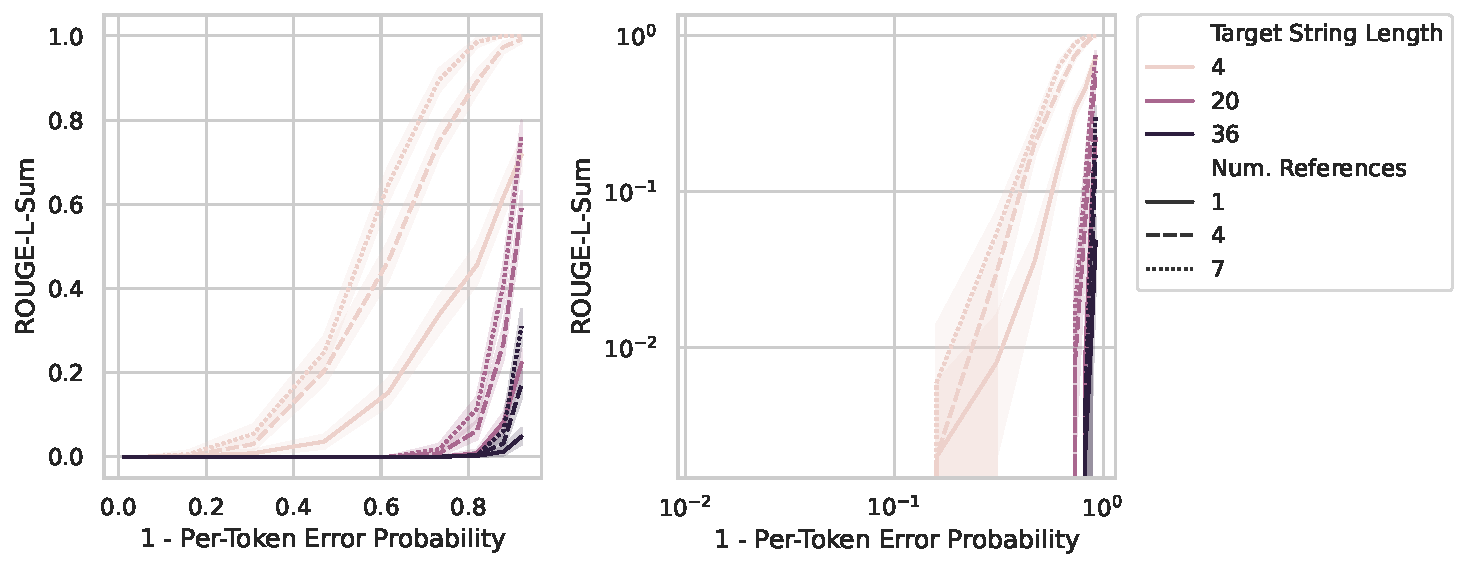
\includegraphics[width=0.95\textwidth]{figures/rouge_understanding/rougeLsum_vs_token_error_prob_scaling_simulation.pdf}
    \caption{\textbf{ROUGE-L-Sum is a sharp metric.} Simulations show that as the per-token error probability slightly increase (e.g. from 0.05 to 0.1), the ROUGE-L-Sum metric sharply falls.}
    \label{fig:app:metric_scaling:rougeLsum}
\end{figure}


Another BIG-Bench metric \cite{srivastava2022beyond} is ROUGE-L-Sum \cite{lin2004rouge}, a metric based on the longest common subsequence (LCS) between two sequences. Section 3.2 of \cite{lin2004rouge} gives the exact definition, but the key property is that ROUGE-L-Sum measures the ``union" LCS, which means ``stitching" together LCSs across the candidate and multiple references. As explained in the original paper: if the candidate sequence is $c = w_1 w_2 w_3 w_4 w_5$, and if there are two reference sequences $r_1 = w_1 w_2 w_6 w_7 w_8$ and $r_2 = w_1 w_3 w_8 w_9 w_5$, then $LCS(r_1, c) = w_1 w_2$ and $LCS(r_2, c) =w_1 w_3 w_5$, then the \textit{union} 
-LCS of $c, r_1, r_2$ is $w_1 w_2 w_3 w_5$, with length 4. Intuitively, this disproportionately benefits models with smaller error rates because their mistakes can be ``stitched" across multiple references; this is confirmed in simulation (Fig. \ref{fig:app:metric_scaling:rougeLsum}).


% \subsection{BLEU}
% \label{app:metric_scaling:bleu}


% \subsection{Emergence does not require on scaling laws: decreasing cross-entropy loss and stricter exact match is all you need }

% The goal of this section is to show that scaling laws are not necessary to create emergence and that many functional forms of the loss are valid as long as the form decreases as some other variable decreases -- say the number of parameters in the model.
% This typically holds in modern machine learning. 
% We do this by considering different functional forms of the cross entropy $CE(N)$, as a function of the number of parameters $N$, and show emergence, i.e. sharpness and unpredictability.
% We illustrate this by showing the programmer can exaggerate the sharpness (and therefore emergence) by implying increasing the exact number of tokens required to get correct in the accuracy, i.e. increasing $L$ in our notation.

% \subsubsection{Argument}

% Recall from section \ref{sec:alt_explanation} the accuracy requiring all $L$ tokens to be correct for a model of size $N$ as a function of cross-entropy $CE(N)$:

% \begin{equation*}
%     \text{Accuracy}(N) \approx p_N(\text{single token correct})^{\text{num. of tokens}} = \exp \Big(- CE(N) \Big)^L
% \end{equation*}

% We plot this equation using three functional forms for a decreasing cross-entropy loss in figure \ref{fig:decreasing_loss_leads_to_emergence_as_L_increases} for increasing values of $L$.
% These increasing values of $L$ induce a sharper -- therefore, seemingly more emergent curve when plotting the accuracy. 
% This means that if the programmer simply requires a stricter accuracy, he can make a perfectly smooth and predictable cross-entropy loss suddenly become sharp and unpredictable, i.e. ``emergent". 
% We show numerically it is independent of the functional form and instead that it only requires the cross-entropy to be decreasing and the accuracy metric to have some non-linear transformation that makes it sharper. 
% Therefore, if one had only tracked the cross-entropy loss instead, one could have had a smooth predictable curve for the models.
% This implies small-scale experimentation is still relevant, and we wish to highly that GPT-4 \cite{gpt4} small-scale experiment in conjunction with scaling loss. 
% We'd like to emphasize that changing the evaluation metric can suddenly induce emergence, and it is not an intrinsic property of the model. 

% %The goal will be to show that if $CE(N)$ decreases with different functional forms that $acc$ is emergent (either sharp or unpredictable).
% % TODO: sharp due to L
% % TODO: unpredictable due to constant and L

% \begin{figure}[htbp]
%   \centering
%   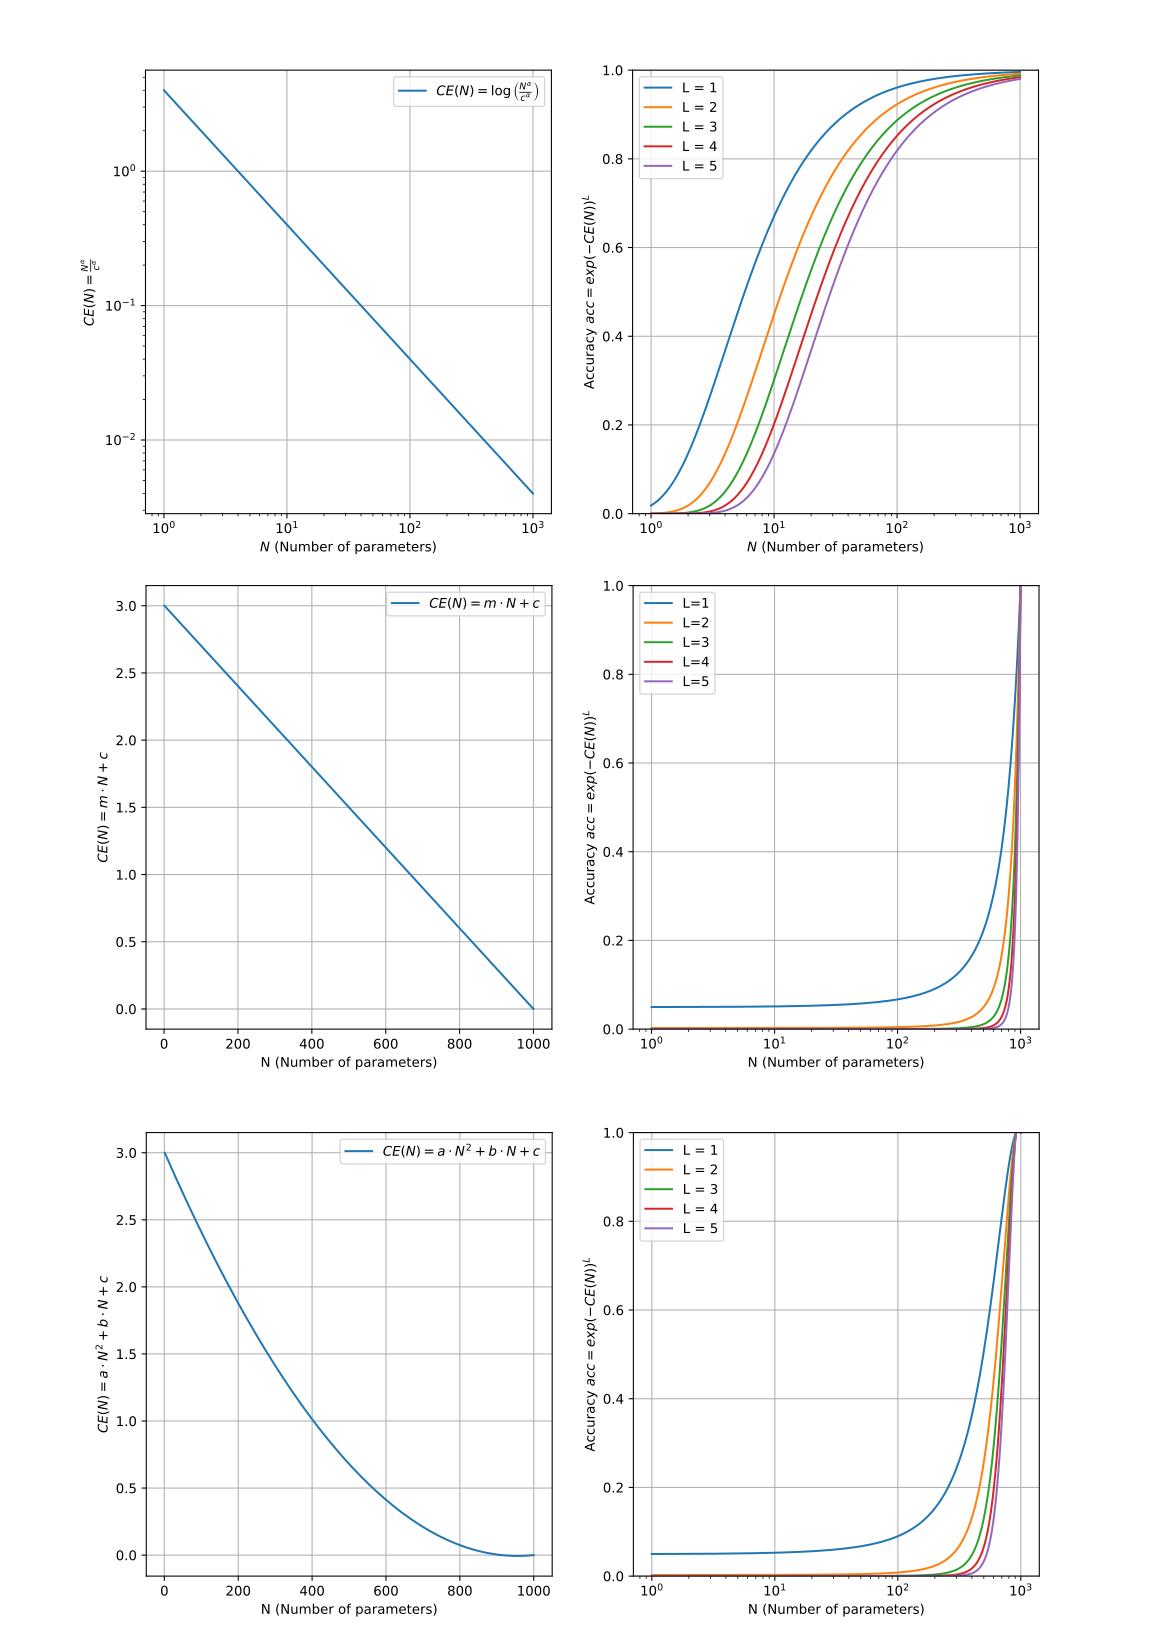
\includegraphics[width=0.8\textwidth]{figures/loss_decreasing_leads_to_emergence/decreasing_loss_leads_to_emergence_as_L_increases.png}
%   \caption{
%   \textbf{Emergence does not depend on scaling laws: any decreasing cross-entropy loss induces apparent emergence as L increases as you require more tokens to be exactly correct, i.e. L increases.}
%   The first row shows the same argument as in the main section, where a decreasing cross-entropy loss as a scaling law induces emergence as $L$ increases.
%   The second row shows the that apparent emergence is induced even when the cross-entropy loss decreases linearly.
%   The third row shows that the apparent emergence is induced when the cross-entropy loss decreases quadratically.
%   Emergence is amplified in this case especially by the increase in sharpness as more tokens are required to be correct. 
%   This means that simply changing the evaluation metric can suddenly induce emergence, and it is not an intrinsic property of the model. 
%   }
%   \label{fig:decreasing_loss_leads_to_emergence_as_L_increases}
% \end{figure}


\section{Inducing Emergent Abilities in Networks on Vision Tasks}
\label{app:sec:inducing_emergence_vision}

\subsection{Emergent Classification of MNIST Handwritten Digits by Convolutional Networks}

\begin{figure}
    \centering
    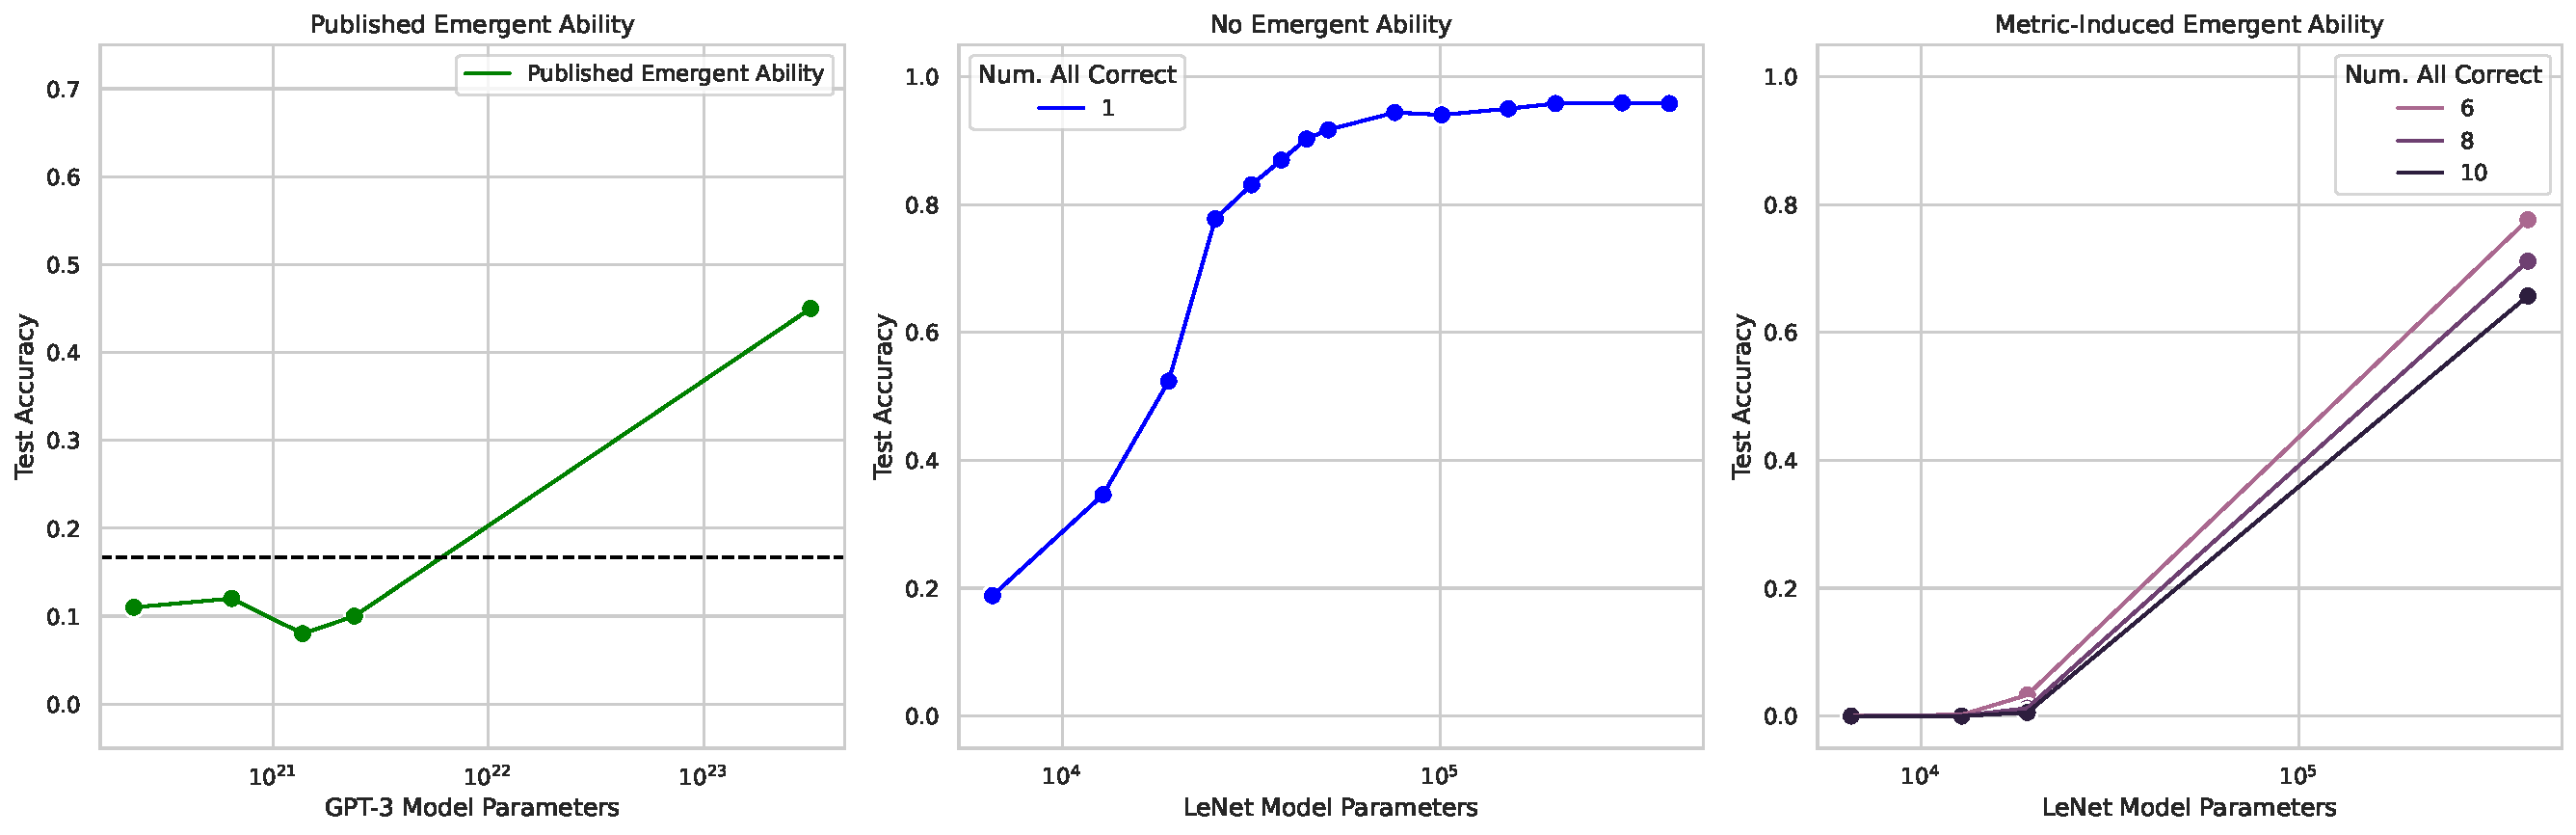
\includegraphics[width=\textwidth]{figures/vision/no_emergence_and_emergence_dataset=mnist.pdf}
    \caption{\textbf{Induced emergent MNIST classification ability in convolutional networks.} (A) A published emergent ability from the BIG-Bench Grounded Mappings task \cite{wei2022emergent}. (B) LeNet trained on MNIST \cite{lecun1998mnist} displays a predictable, commonplace sigmoidal increase in test accuracy as model parameters increase. (C) When accuracy is redefined as correctly classifying $K$ out of $K$ independent test data, this newly defined metric induces a seemingly unpredictable change.}
    \label{fig:vision_mnist}
\end{figure}

We begin by inducing an emergent classification ability in a LeNet convolutional neural network family \cite{lecun1998gradient}, trained on the MNIST handwritten digits dataset \cite{lecun1998mnist}.
This family displays smoothly increasing test accuracy as the number of parameters increase (Fig. \ref{fig:vision_mnist}B).
To emulate the accuracy metric used by emergence papers \cite{ganguli2022predictability, wei2022emergent, srivastava2022beyond}, we use \textit{subset accuracy}: 1 if the network classifies $K$ out of $K$ (independent) test data correctly, 0 otherwise.
Under this definition of accuracy, the model family displays an ``emergent" ability to correctly classify sets of MNIST digits as $K$ increases from $1$ to $5$, especially when combined with sparse sampling of model sizes (Fig. \ref{fig:vision_mnist}C).
This convolutional family's emergent classification ability qualitatively matches published emergent abilities, e.g., at the BIG-Bench Grounded Mappings task \cite{wei2022emergent} (Fig. \ref{fig:vision_mnist}A).


\end{document}
